\documentclass[12pt]{book}
\usepackage[a4paper,width=150mm,top=25mm,bottom=25mm]{geometry}         
\usepackage{amsmath}        
\usepackage{graphicx}        
\usepackage{xcolor}
\usepackage{float}
\usepackage{titlesec}
\usepackage{subcaption}
\usepackage{multicol}
\usepackage{enumitem}
\usepackage{setspace}
\usepackage{mdframed}
\usepackage{hyperref}
\usepackage{listings}
\usepackage[italian]{babel}
\usepackage{minted}
%\setlist{nosep}
    
\definecolor{lightgray}{gray}{0.95}    
    
% Stile dei titoli dei capitoli    
\definecolor{gray75}{gray}{0.75}    
\newcommand{\hsp}{\hspace{20pt}}    
\titleformat{\chapter}[hang]    
{\Huge\bfseries}    
{\thechapter\hsp\textcolor{gray75}{|}\hsp}    
{0pt}    
{\Huge\bfseries}    

\newenvironment{multicolfigure}
  {\par\medskip\noindent\minipage{\linewidth}}
  {\endminipage\par\medskip}

\onehalfspacing
\begin{document}

\tableofcontents

\chapter{Linguaggi, macchine astratte, teoria della computabilità}

\subsubsection{Alcune definizioni}
\begin{itemize}
    \item \textbf{Algoritmo}: sequenza \textit{finita} di istruzioni che risolve in un \textit{tempo finito} una classe di problemi
    \item \textbf{Codifica}: descrizione dell'algoritmo tramite un \textit{insieme ordinato di frasi} di un linguaggio di programmazione, che specificano le \textit{azioni} da svolgere
    \item \textbf{Programma}: testo scritto in accordo alla \textit{sintassi} e alla \textit{semantica} di un linguaggio di programmazione
\end{itemize}

\subsection{Esecuzione}
Un algoritmo esprime la soluzione a un problema, il programma è la formulazione testuale rigorosa in un dato linguaggio; l'esecuzione \textit{ordinata} delle azioni specificate porta a ottenere la soluzione da un insieme di dati in ingresso.

Viene assunta l'esistenza di un \textbf{automa esecutore}, una macchina astratta capace di eseguire le azioni dell'algoritmo.

\begin{figure}[H]
    \centering
    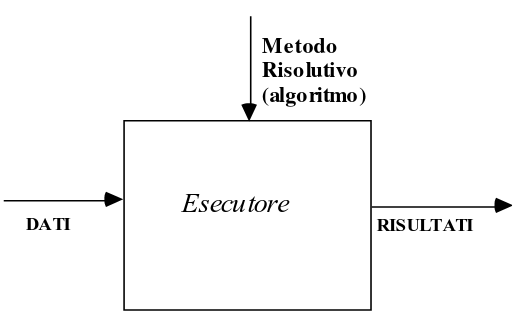
\includegraphics[width=0.6\textwidth]{/home/riccardoob/appunti/linguaggi/images/26.png}
\end{figure}

\section{Macchine astratte}

\subsection{Automa esecutore}
Un automa deve poter ricevere dall'esterno una \textit{descrizione} dell'algoritmo, deve quindi essere in grado di \textit{interpretare} un linguaggio, che verrà chiamato \textbf{linguaggio macchina}.

\subsubsection{Realizzabilità fisica}
\begin{itemize}
    \item le parti che compongono l'automa devono essere in \textit{numero finito}
    \item ingresso e uscita devono essere denotabili da un \textit{insieme finito} di \textbf{simboli}
\end{itemize}

\subsection{Gerarchia di macchine astratte}
\begin{itemize}
    \item macchina combinatoria
    \item automi a stati finiti
    \item ....
    \item macchina di Turing
\end{itemize}

Si individua una gerarchia perché diverse classi di macchina hanno diversa \textit{capacità} di risolvere problemi. Se neanche la macchina più "potente" può risolvere un problema, questo potrebbe essere \textbf{non risolubile}.

\subsection{Macchina base}
La macchina base è definita formalmente dalla tripla:
\begin{equation*}
    \langle I, O, mfn\rangle
\end{equation*}
dove
\begin{itemize}
    \item $I$ = insieme finito dei simboli di \textit{ingresso}
    \item $O$ = insieme finito dei simboli di \textit{uscita}
    \item $mfn: I \rightarrow O$ = funzione di macchina
\end{itemize}

\subsubsection{Limiti}
Utilizzare una di queste macchine per risolvere problemi comporta valutare tutte le possibili configurazioni di ingresso.

Esiste inoltre un altro limite, essendo puramente combinatoria, la macchina base non può risolvere problemi che richiedano di ricordare qualcosa dal passato, in quanto privo di memoria interna.

\subsection{Automa a stati finiti}
Nell'automa a stati finiti si introduce il concetto di memoria attraverso l'utilizzo di un numero \textit{finito} di \textbf{stati interni}.

Un \textbf{automa a stati finiti} è definito dalla quintupla:
\begin{equation*}
    \langle I, O, S, mfn, sfn\rangle
\end{equation*}
dove
\begin{itemize}
    \item $I$ = insieme finito dei simboli di \textit{ingresso}
    \item $O$ = insieme finito dei simboli di \textit{uscita}
    \item $mfn: I \times S \rightarrow O$ = funzione di macchina
    \item $sfn: I \times S \rightarrow S$ = funzione di \textbf{stato}
\end{itemize}

\subsubsection{Limiti}
Dato che lo stato funge da memoria interna, le risposte possono essere diverse a parità di dati d'ingresso.

Esistono varie categorie ASF come automi di Mealy o Moore, sincroni o asincroni, minimo numero di stati etc..

Esiste un limite computazionale che rende l'automa inadatto a risolvere problemi che non permette di limitare a priori la lunghezza delle sequenze, dovuto al fatto che la memoria è \textbf{finita}.

\subsection{Macchina di Turing}
Per ovviare al limite della memoria finita, si introduce un \textit{nastro} di memoria esterno, la \textbf{macchina di Turing} è definita dalla quintupla:
\begin{equation*}
    \langle A, S, mfn, sfn, dfn\rangle
\end{equation*}
dove
\begin{itemize}
    \item $A$ = insieme finito dei simboli di \textit{ingresso} e \textit{uscita}
    \item $S$ = insieme finito degli \textit{stati} (tra i quali \textit{HALT})
    \item $mfn: A \times S \rightarrow A$ = funzione di macchina
    \item $sfn: A \times S \rightarrow S$ = funzione di stato
    \item $dfn: A \times S \rightarrow D$ = $\{Left, Right, None\}$, funzione di \textit{direzione}
\end{itemize}

Il deposito dei dati è rappresentato da un natro illimitatamente espandibile
\begin{figure}[H]
    \centering
    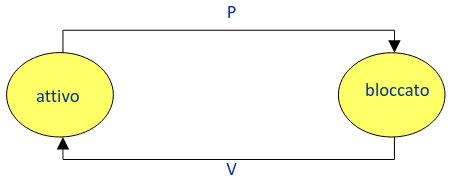
\includegraphics[width=0.8\textwidth]{/home/riccardoob/appunti/linguaggi/images/27.png}
\end{figure}

La macchina è dotata di una testina di lettura e scrittura che può:
\begin{itemize}
    \item leggere un simbolo dal nastro
    \item scrivere sul nastro il simbolo specificato da $mfn()$
    \item passare a un nuovo stato interno specificato dalla $sfn()$
    \item spostarsi sul nastro di una posizione nella direzione indicata da $dfn()$
\end{itemize}
ipotizzando che quando viene raggiunto lo stato HALT, la macchina si ferma.

Per risolvere un problema con questa macchina, è necessario definire la \textit{rappresenzatione dei dati} di partenza (da porre sul nastro) e quelli di uscita (sempre sul nastro), e definire il \textit{comportamento}, ovvero le tre funzioni $mfn()$, $sfn()$ e $dfn()$.

Non è certo che questa macchina arrivi allo stato di HALT.

\subsubsection{Tesi di Church-Turing}
Esiste una macchina più "potente" della MdT?

La tesi di Church-Turing afferma che
\begin{mdframed}[topline=false,bottomline=false,rightline=false]
    Non esiste alcun formalismo capace di risolvere una classe di problemi più ampia di quella risolta dalla macchina di Turing.
\end{mdframed}

\subsection{Macchine universali}
Nella macchina di Turing l'algoritmo è cablato nella macchina.

Si può espandere la MdT alla macchina di Turing \textbf{Universale} (UTM), macchina il cui programma è letto dalla macchina direttamente dal nastro.

Questo richiede poter descrivere l'algoritmo richiesto attraverso un \textit{linguaggio} e avere una macchina che lo interpreti.

Le tre operazioni che la UTM effettua sono:
\begin{itemize}
    \item \textbf{fetch}, ricerca delle istruzioni
    \item \textbf{decode}, interpretazione delle istruzioni
    \item \textbf{execute}, esecuzione le istruzioni
\end{itemize}

\subsubsection{UTM vs Macchina di Von Neumann}

\begin{multicols}{2}
    \noindent
    Macchina di Turing
    \begin{itemize}
        \item leggere/scrivere simbolo da/su nastro
        \item transitare in un nuovo stato
        \item spostarsi sul nastro di x posizioni
    \end{itemize}
    \columnbreak
    \begin{mdframed}[topline=false,bottomline=false,rightline=false] 
        Macchina di Von Neumann
        \begin{itemize}
            \item lettura/scrittura da/su RAM/ROM
            \item nuova configurazione registri CPU
            \item scelta cella di memoria su cui operare
        \end{itemize}
    \end{mdframed}
\end{multicols}

La UTM non ha il concetto di "mondo esterno", ne nessuna istruzione di I/O, è puramente computazione senza la dimensione di \textit{interazione}.

\subsubsection{Computazione e interazione}
Computazione e interazione sono dimensioni \textit{ortogonali}, potenzialmente espressi da due linguaggi distinti:
\begin{multicols}{2} 
    \begin{itemize}
        \item linguaggio di \textbf{computazione}
        \item linguaggio di \textbf{coordinazione}
        \begin{itemize}
            \item linguaggio di \textbf{comunicazione}
        \end{itemize}
    \end{itemize}
    \begin{mdframed}[topline=false,bottomline=false,rightline=false]
        \begin{multicolfigure}
            \centering
            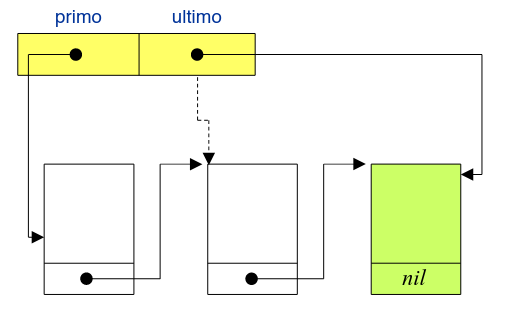
\includegraphics[width=0.6\textwidth]{/home/riccardoob/appunti/linguaggi/images/28.png}
        \end{multicolfigure}
    \end{mdframed}
\end{multicols}

\section{Teoria della computabilità}

\subsubsection{Problemi irrisolubili}
Secondo la tesi di Church-Turing, non esiste un formalismo più potente della macchina di Turing, quindi se la MdT non riesce a risolvere un problema, quel problema è \textbf{irrisolubile}.

Per irrisolubile si intende che la MdT non si ferma, quindi non ritorna un output definito.

\subsubsection{Problemi risolubili}
Un problema risolubile è un problema la cui soluzione può essere calcolata da una MdT o equivalenti.

\section{Funzioni}
Per valutare la risolubilità di un problema è necessario individuare una \textbf{funzione} che lo descrive.

\subsection{Funzione caratteristica}
Come prima cosa si definisce la funziona \textbf{caratteristica} di un problema.

\begin{mdframed}[topline=false,bottomline=false,rightline=false]
    Dato un problema $P$ e detti
    \begin{itemize}
        \item $X$ l'insieme dei suoi dati in ingresso
        \item $Y$ l'insieme delle risposte corrette
    \end{itemize}
    si dice funzione caratteristica del problema $P$
    \begin{equation*}
        f_p: X \rightarrow Y
    \end{equation*}
\end{mdframed}

In questo modo, problema non risolubile equivale a una funzione caratteristica non computabile.

\subsection{Funzione computabile}
Si formalizza ora la classe di funzioni dette \textbf{computabili}.

\begin{mdframed}[topline=false,bottomline=false,rightline=false]
    Una funzione $f:A \rightarrow B$ è detta \textit{computabile} se esiste una macchina di Turing che, data sul nastro una rappresentazione di $x \in A$, dopo un \textit{numero finito} di passi produce sul nastro una rappresentazione di $f(x) \in B$.
\end{mdframed}

\subsection{Funzioni definibili vs funzioni computabili}
É necessario capire se tutte le funzioni sono computabili, o se esistono funzioni definibili ma non computabili.

\subsubsection{Funzione computabile su N}
Per semplicità, considereremo funzioni sui \textit{numeri naturali}
\begin{equation*}
    f: N \rightarrow N
\end{equation*}
Questa condizione non è limitativa, dato che ogni informazione è necessariamente finita, può quindi essere codificata con una collezione di numeri naturali, la quale a sua volta può essere espressa tramite un \textit{unico} numero naturale (procedimento di Gödel.

\subsubsection{Procedimento di Gödel}
Data una collezione di numeri naturali, ottenere un unico numero naturale.

\begin{mdframed}[topline=false,bottomline=false,rightline=false]
    \begin{itemize}
        \item siano $N_1, N_2, \dots, N_k$ i numeri naturali dati
        \item siano $P_1, P_2, \dots, P_k$ i primi $k$ numeri primi
    \end{itemize}
    Si definisce $R$, un nuovo numero naturale così definito
    \begin{equation*}
        R ::= P_1^{N_1} \cdot P_2^{N_2} \cdot \dots \cdot P_k^{N_k}
    \end{equation*}
\end{mdframed}
R rappresenta unicamente la collezione originale $N_1, N_2, \dots, N_k$.

Poiché che l'insieme $F=\{f: N \rightarrow N\}$ delle funzioni sui naturali non è \textit{enumerabile}, e l'insieme delle funzioni computabili è enumerabile (dato che l'insieme dei simboli è finito ogni MdT può essere associata a un numero di Gödel), la gran parte delle funzioni definibili \underline{non è computabile}.

Interessano però soltanto le funzioni definibili con un linguaggio basato su un alfabeto finito di simboli, sfortunamtamento esistono funzioni definibili con tale alfabeto ma \textit{non computabili}.

\subsection{Funzioni non computabili}
Dire che esistono funzioni definibili ma non computabili, equivale a dire che esistono problemi irrisolubili, basta trovare uno solo di questi problemi.

\subsubsection{Problema dell'HALT della macchina di Turing}
\begin{mdframed}[topline=false,bottomline=false,rightline=false]
    Stabilire se una data macchina di Turing T, con un generico ingresso X, si ferma oppure no.
\end{mdframed}

Slide 49-55.

\subsection{Generabilità e decidibilità}
Poiché un linguaggio è un insieme di frasi, è utile indagare la \textbf{generabilità} e la \textbf{decidibilità} di un insieme.

Si introduce il concetto di \textit{insieme ricorsivamente numerabile}, per decidere che l'insieme sia effettivamente generabile.

\subsubsection{Insieme ricorsivamente numerabile}
Data la definizione di un insieme numerabile, ovvero un insieme i cui elementi possono essere "contati" cioè che possiede una funzione biettiva:
\begin{equation*}
    f: N \rightarrow S
\end{equation*}
che mette in corrispondenza i numeri naturali con gli elementi del sistema.

Si passa alla definizione di insieme \textbf{ricorsivamente numerabile} (\textit{semi-decidibile}). 
\begin{mdframed}[topline=false,bottomline=false,rightline=false]
    Un insieme è ricorsivamente numerabile se la funzione biettiva $f: N \rightarrow S$ è \textit{computabile}.
\end{mdframed}
\begin{figure}[H]
    \centering
    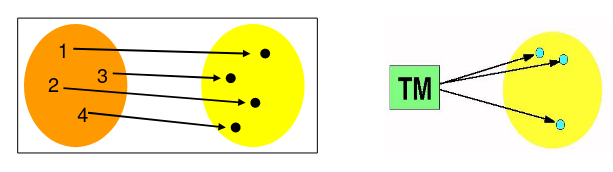
\includegraphics[width=0.6\textwidth]{/home/riccardoob/appunti/linguaggi/images/29.png}
\end{figure}
Tuttavia, il fatto che l'insieme possa essere costruito, non significa che si possa decidere se un certo elemeto vi appertiene o no.

\subsubsection{Decidibilità}
In generale, da un insieme ricorsivamente numerabile, potrebbe non essere trovabile un elemento, in questo caso la MdT può entrare in loop:
\begin{mdframed}[topline=false,bottomline=false,rightline=false]
    Un inisieme è \textbf{semi-decidibile} se è possibile stabilire se un elemento appartiene a un insieme ma non se un elemento \textit{non appartiene}.
\end{mdframed}

\subsection{Insiemi decidibili}
Occore un concetto più potente della semi-decidibilità.
\begin{mdframed}[topline=false,bottomline=false,rightline=false]
    Un insieme $S$ è \textbf{decidibile} (o ricorsivo) se la sua funzione caratteristia è computabile.
    \begin{equation*}
        f(x) = 
        \begin{cases}
            1, \text{se } x \in S\\
            0, \text{se } x \notin S
        \end{cases}
    \end{equation*}
\end{mdframed}

ovvero se esiste una macchina di Turing capace di rispondere sì o no, senza mai entrare in un \textit{ciclo infinito}, alla domanda se un certo elemento appartiene all'insieme.

\begin{mdframed}[topline=false,bottomline=false,rightline=false]
    \textbf{Teorema 1}\\
    Se un insieme è \textbf{decidibile} è anche \textbf{semi-decidibile}, ma non viceversa.
\end{mdframed}

\begin{mdframed}[topline=false,bottomline=false,rightline=false]
    \textbf{Teorema 2}\\
    Un insieme $S$ è \textbf{decidibile} se e solo se
    \begin{itemize}
        \item $S$
        \item il suo complemento $N-S$
    \end{itemize}
    sono \textbf{semi-decidibili}.
\end{mdframed}


\chapter{Linguaggi e grammatiche}
empty

\chapter{Riconoscitori a stati finiti}
...
\section{Dai riconoscitori ai generatori}
\begin{figure}[H]
    \caption{Automa}
    \centering
    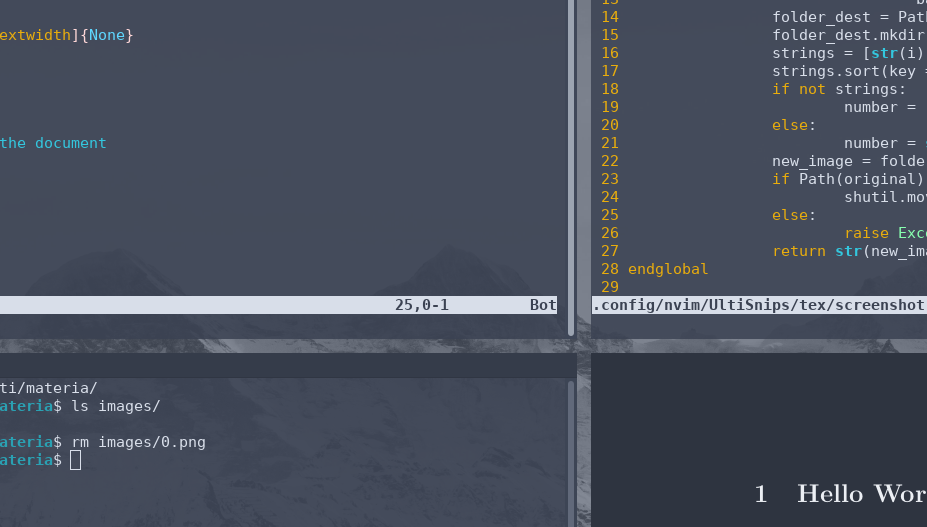
\includegraphics[width=0.8\textwidth]{/home/riccardoob/appunti/linguaggi/images/0.png}
\end{figure}

Descrivendo a parole le transizioni utili dell'automa:
\begin{itemize}
    \item nello stato I l'automa può accettare:
    \begin{itemize}
        \item il simbolo a e portarsi nello stato A
    \end{itemize}
    \item nello stato A l'automa può accettare:
    \begin{itemize}
        \item il simbolo b e poi fermarsi
        \item il simbolo a e riportarsi nello stato A stesso
    \end{itemize}
    \item nello stato finale F l'automa puà accettare:
    \begin{itemize}
        \item nessun simbolo
    \end{itemize}
\end{itemize}

Se si sostituisce la parola accettare alla parola generare, si nota che l'automa può essere considerato come generatore.

Si può definire un \textbf{mapping} tra:
\begin{itemize}
    \item stati $\longleftrightarrow$ simboli non terminali
    \item transizioni $\longleftrightarrow$ produzioni
    \item scopo $\longleftrightarrow$ uno stato particolare
\end{itemize}

É possibile automatizzare la costruzione di un RSF a partire dalla grammatica o viceversa.

\begin{multicols}{2}
Grammatica regolare a \underline{destra}:
\begin{itemize}
    \item scopo = stato iniziale: $I$
    \item stato finale: $F$
    \begin{itemize}
        \item $S \rightarrow a\ A$
        \item $A \rightarrow a\ A\ |\ b$
    \end{itemize}
\end{itemize}
Grammatica regolare a \underline{sinistra}:
\begin{itemize}
    \item scopo = stato finale: $F$
    \item stato inziale: $I$
    \begin{itemize}
        \item $S \rightarrow A\ b$
        \item $A \rightarrow A\ a\ |\ a$
    \end{itemize}
\end{itemize}
\end{multicols}

Lo stato finale F non si considera perché non ha archi uscenti.

Come arrivare a queste grammatiche?

\subsection{Mapping RSF $\longleftrightarrow$ grammatica}

Si immagini un osservatore che, stando in ogni stato, guardi da ogni stato:

\begin{multicols}{2}
    \begin{itemize}
        \item \underline{dove si va}
        \begin{itemize}
            \item la freccia col \textbf{simbolo terminale}
            \item lo stato \textbf{successivo}
        \end{itemize}
        \item \underline{da dove viene}
        \begin{itemize}
            \item lo stato \textbf{precendente}
            \item la freccia col \textbf{simbolo terminale}
        \end{itemize}
    \end{itemize}
\end{multicols}

\subsubsection{Mapping tra automa riconoscitore e grammatica}
Tra la grammatica e il riconoscitori si riconoscono le seguenti corrispondenze:
\begin{itemize}
    \item \textbf{stati} dell'automa $\longleftrightarrow$ \textbf{metasimboli} della grammatica
    \item \textbf{transizioni} dell'automa $\longleftrightarrow$ \textbf{produzioni} della grammatica
    \item \textbf{uno stato} dell'automa $\longleftrightarrow$ \textbf{scopo} della grammatica
\end{itemize}
Se la grammatica è \underline{regolare a destra} si ottiene un automa \underline{top-down}.\\
Se la grammatica è \underline{regolare a sinistra} si ottiene un automa \underline{bottom-up}.\\
In modo analogo si ottengono grammatiche destra/sinistra interpretando un RSF in modo top-down/bottom-up

\noindent
Ad esempio:

In questo caso gli stati iniziale e finale sono anche \underline{stati di transito}.
\begin{figure}[H]
    \begin{subfigure}{0.5\textwidth}
        \caption{Traduzione grammatica}
        \centering
        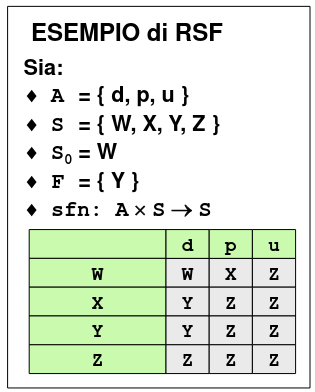
\includegraphics[width=0.4\linewidth]{/home/riccardoob/appunti/linguaggi/images/1.png}
    \end{subfigure}% 
    \begin{subfigure}{0.5\textwidth}
        \caption{Riconoscitore}
        \centering
        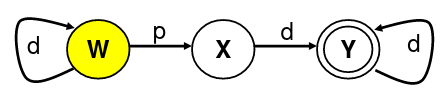
\includegraphics[width=0.4\linewidth]{/home/riccardoob/appunti/linguaggi/images/2.png}
    \end{subfigure}
\end{figure}

Per passare dall'automa alla grammatica si analizzano i collagamenti degli stati e si ricavano le trasformazioni:
\\
\begin{multicols}{2}
    \noindent
    \begin{equation*}
        \begin{aligned}[t]
        &W \rightarrow d\ W &&|\ p\ X\\
        &X \rightarrow d\ &&|\ d\ Y\\
        &Y \rightarrow d\ &&|\ d\ Y
        \end{aligned}
    \end{equation*}
    \begin{equation*}
        \begin{aligned}[t]
        &Y \rightarrow X\ d &&|\ Y\ d\\
        &X \rightarrow p\ &&|\ W\ p\\
        &W \rightarrow d\ &&|\ W\ d
        \end{aligned}
    \end{equation*}    
\end{multicols}

\subsection{Riconoscitori top down}
\textbf{Derivazione top-down}\\
si parte dallo scopo della grammatica e si tenta di coprire la frase data tramite produzioni successive.\\
\begin{multicols}{2}
Data una grammatica regolare lineare a \underline{destra}, il riconoscitore:
\begin{itemize}
    \item ha tanti \textbf{stati} quanti i \underline{simboli non terminali}
    \item ha come \textbf{stato iniziale} lo \underline{scopo S}
    \item per ogni regola del tipo $X \rightarrow x\ Y$, l'automa con ingresso $x$ passa dallo stato $X$ allo stato $Y$
    \item per ogni regola del tipo $X \rightarrow x$, l'automa con ingresso $x$ passa dallo stato $X$ allo stato finale $F$
\end{itemize}
\columnbreak
\textbf{Esempio}\\
Sia G una grammatica lineare a destra caratterizzata dalle seguenti produzioni:
\begin{itemize}
    \item $S \rightarrow a\ B\ |\ b$
    \item $B \rightarrow b\ S\ |\ a$
\end{itemize}
\begin{multicolfigure}
    \centering
    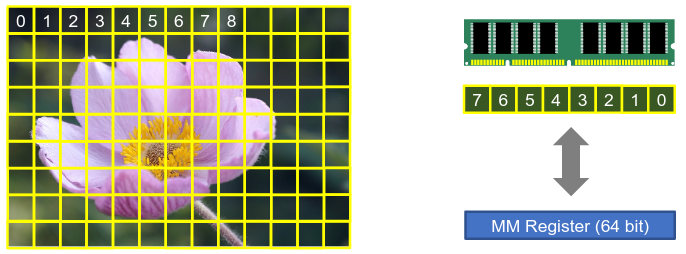
\includegraphics[width=0.4\textwidth]{/home/riccardoob/appunti/linguaggi/images/3.png}
\end{multicolfigure}
\end{multicols}

\subsection{Riconoscitori bottom up}
\begin{multicols}{2}
Data una grammatica regolare lineare a \underline{sinistra}, il riconoscitore:
\begin{itemize}
    \item ha tanti \textbf{stati} quanti i \underline{simboli non terminali}
    \item ha come \textbf{stato finale} lo \underline{scopo S}
    \item per ogni regola del tipo $X \rightarrow Y\ x$, l'automa con ingresso $x$ passa dallo stato $Y$ allo stato $X$
    \item per ogni regola del tipo $X \rightarrow x$, l'automa con ingresso $x$ passa dallo stato iniziale $I$ allo stato $X$
\end{itemize}
\columnbreak
\textbf{Esempio}\\
Sia G una grammatica lineare a sinistra caratterizzata dalle seguenti produzioni:
\begin{itemize}
    \item $S \rightarrow B\ a\ |\ b$
    \item $B \rightarrow S\ b\ |\ a$
\end{itemize}
\begin{multicolfigure}
    \centering
    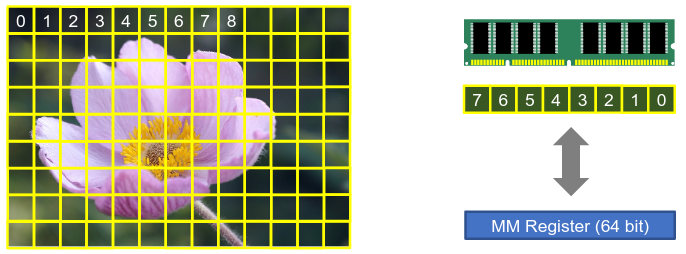
\includegraphics[width=0.4\textwidth]{/home/riccardoob/appunti/linguaggi/images/3.png}
\end{multicolfigure}
\end{multicols}

\subsection{Dall'automa alle grammatiche}
Dato un automa riconoscitore, se ne possono trarre sia una grammatica regolare a \underline{destra} (interpretazione top-down) che una grammatica regolare a \underline{sinistra} (interpretazione bottom-up).
\noindent\\
\begin{multicols}{2} 
Caso generico
\begin{itemize}
    \item top-down:     $A \rightarrow a\ B$
    \item bottom-up:     $A\ a \leftarrow B$
\end{itemize}    
\columnbreak
\begin{multicolfigure}
    \centering
    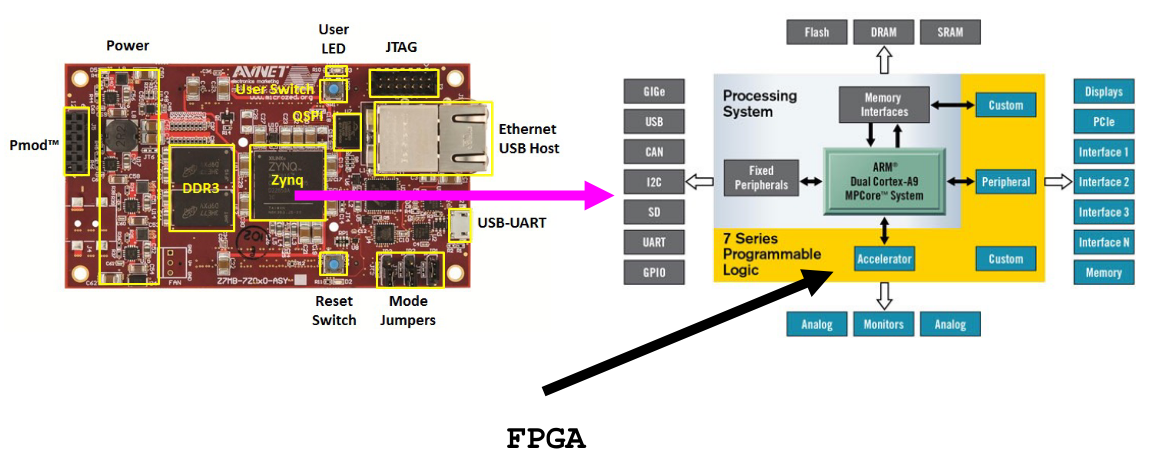
\includegraphics[width=0.5\textwidth]{/home/riccardoob/appunti/linguaggi/images/6.png}
\end{multicolfigure}
\end{multicols}
\begin{multicols}{2}
    \noindent
    Caso iniziale
    \begin{itemize}
        \item top-down:     $S \rightarrow a\ B$
        \item bottom-up:    $I\ a \leftarrow B$
    \end{itemize}
    \begin{multicolfigure}
        \centering
        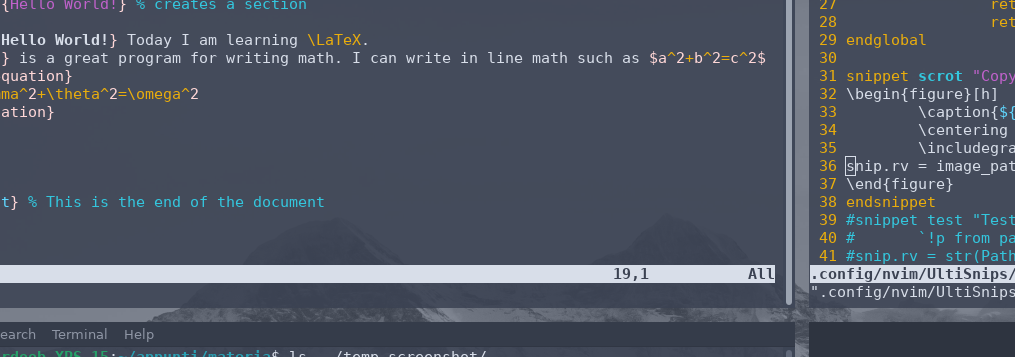
\includegraphics[width=0.5\textwidth]{/home/riccardoob/appunti/linguaggi/images/4.png}
    \end{multicolfigure}
    \columnbreak
    \noindent
    Caso finale
    \begin{itemize}
        \item top-down:     $A \rightarrow a\ F$
        \item bottom-up:    $A\ a \leftarrow S$
    \end{itemize}
    \begin{multicolfigure}
        \centering
        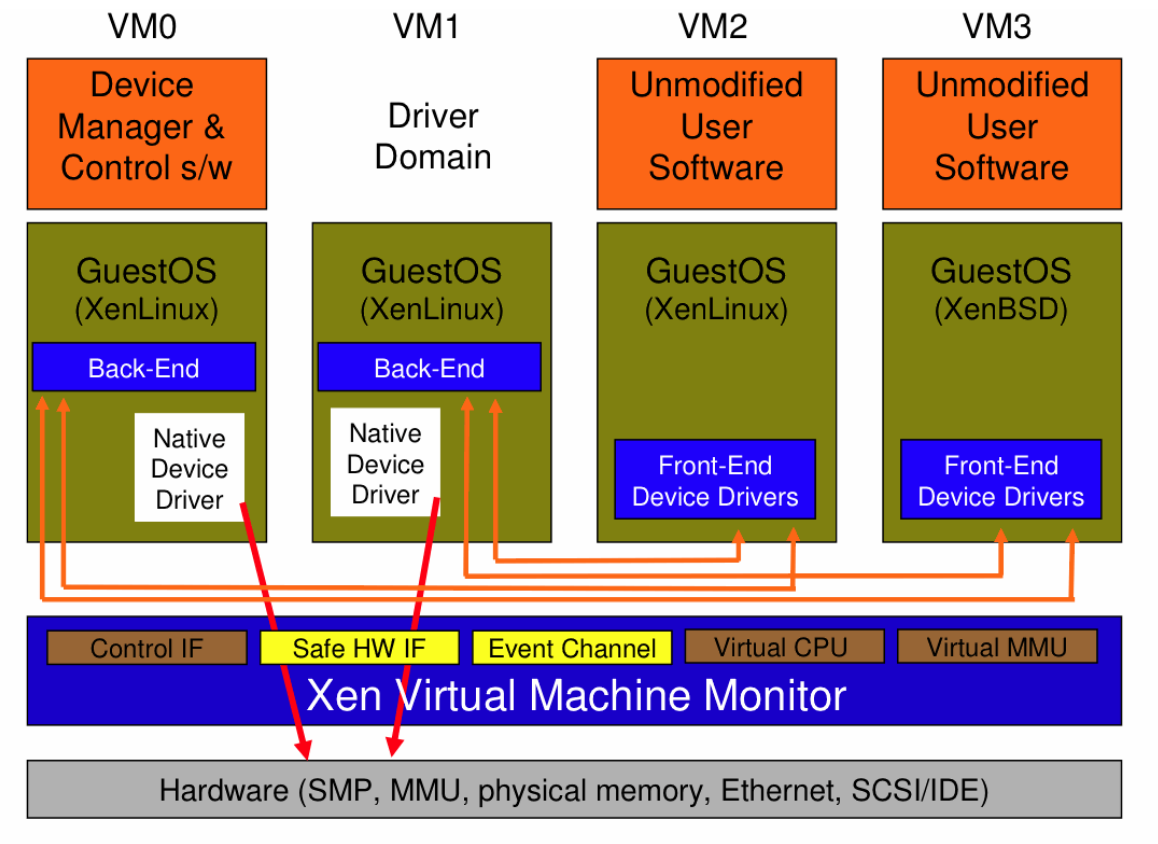
\includegraphics[width=0.5\textwidth]{/home/riccardoob/appunti/linguaggi/images/5.png}
    \end{multicolfigure}
\end{multicols}

\subsubsection{Esempio}

\begin{figure}[H]
    \centering
    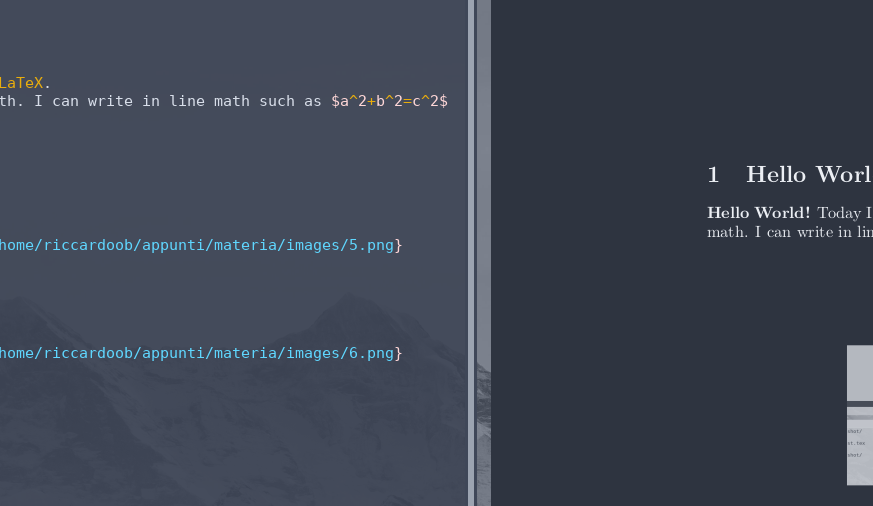
\includegraphics[width=0.4\textwidth]{/home/riccardoob/appunti/linguaggi/images/7.png}
\end{figure}

\setlist{nosep}
\begin{multicols}{2}
\noindent
Analisi top-down (C finale omesso):
\begin{itemize}
    \item $I \rightarrow b\ B$
    \item $I \rightarrow a\ A$
    \item $B \rightarrow a\ A$
    \item $A \rightarrow a\ A$
    \item $B \rightarrow c$
    \item $A \rightarrow c$
\end{itemize}

\columnbreak
\noindent
Analisi bottom-up (C iniziale):
\begin{itemize}
    \item $b \leftarrow  B$
    \item $a \leftarrow  A$
    \item $B\ a \leftarrow  A$
    \item $A\ a \leftarrow  A$
    \item $B\ c \leftarrow  S$
    \item $A\ c \leftarrow  S$
\end{itemize}
\end{multicols}
\setlist{}

\begin{multicols}{2}
\noindent
Grammatica G1 regolare a destra:
\begin{itemize}
    \item $I \rightarrow b\ B\ |\ a\ A$
    \item $B \rightarrow a\ A\ |\ c$
    \item $A \rightarrow a\ A\ |\ c$
\end{itemize}
\begin{multicolfigure}
    \centering
    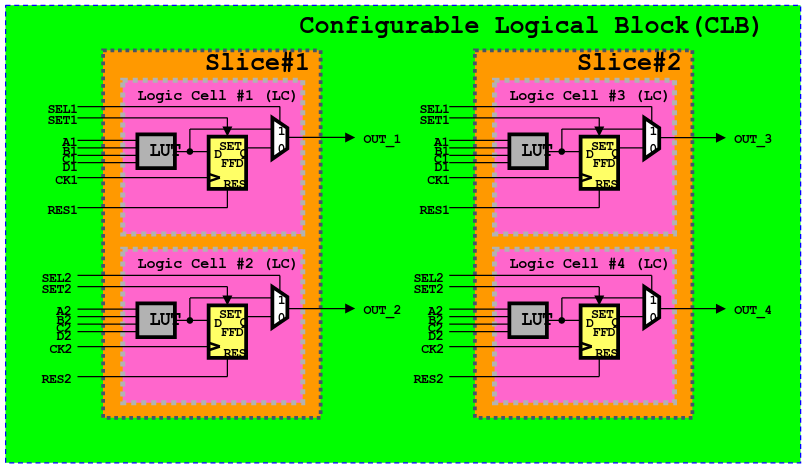
\includegraphics[width=0.7\textwidth]{/home/riccardoob/appunti/linguaggi/images/8.png}
\end{multicolfigure}
\columnbreak
\noindent
Grammatica G2 regolare a sinistra:
\begin{itemize}
    \item $S \rightarrow B\ c\ |\ A\ c$
    \item $A \rightarrow B\ a\ |\ A\ a\ |\  a$
    \item $B \rightarrow b$
\end{itemize}
\begin{multicolfigure}
    \centering
    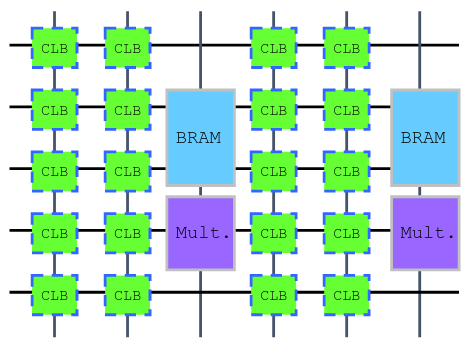
\includegraphics[width=0.7\textwidth]{/home/riccardoob/appunti/linguaggi/images/9.png}
\end{multicolfigure}    
\end{multicols}

\textbf{Esempio multipli stati finali}\\
\begin{figure}[H]
    \centering
    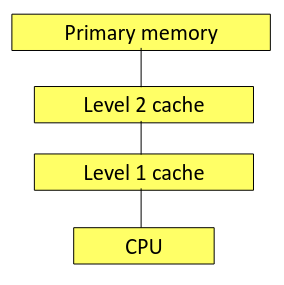
\includegraphics[width=0.4\textwidth]{/home/riccardoob/appunti/linguaggi/images/10.png}
\end{figure}

\setlist{nosep}
\begin{multicols}{2}
\noindent
Analisi top-down (regola in più sulla $I$):
\begin{itemize}
    \item $I \rightarrow b\ B\ |\ b$
    \item $I \rightarrow a\ A$
    \item $B \rightarrow a\ A$
    \item $A \rightarrow a\ A$
    \item $B \rightarrow c$
    \item $A \rightarrow c$
\end{itemize}

\columnbreak
\noindent
Analisi bottom-up (C iniziale):
\begin{itemize}
    \item $b \leftarrow  B$
    \item $a \leftarrow  A$
    \item $B\ a \leftarrow  A$
    \item $A\ a \leftarrow  A$
    \item $B\ c \leftarrow  C$
    \item $A\ c \leftarrow  C$
\end{itemize}
\end{multicols}
\setlist{}
L'analisi bottom-up deve scegliere quale scopo adottare, se $B$ o $C$. Per risolvere questo problema si creano due grammatiche in cui si assumono a turno $C \equiv S$ e $B \equiv S$.


\begin{figure}[H]
    \begin{subfigure}{0.5\textwidth}
        \centering
        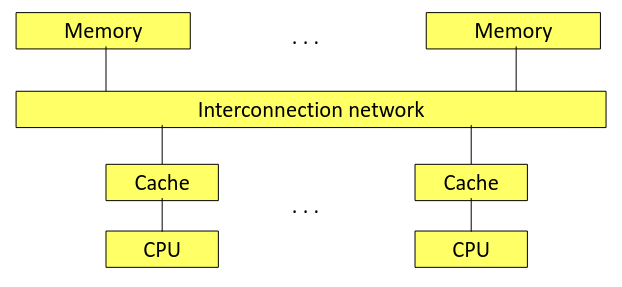
\includegraphics[width=0.7\linewidth]{/home/riccardoob/appunti/linguaggi/images/11.png}
    \end{subfigure}%
    \begin{subfigure}{0.5\textwidth}
        \centering
        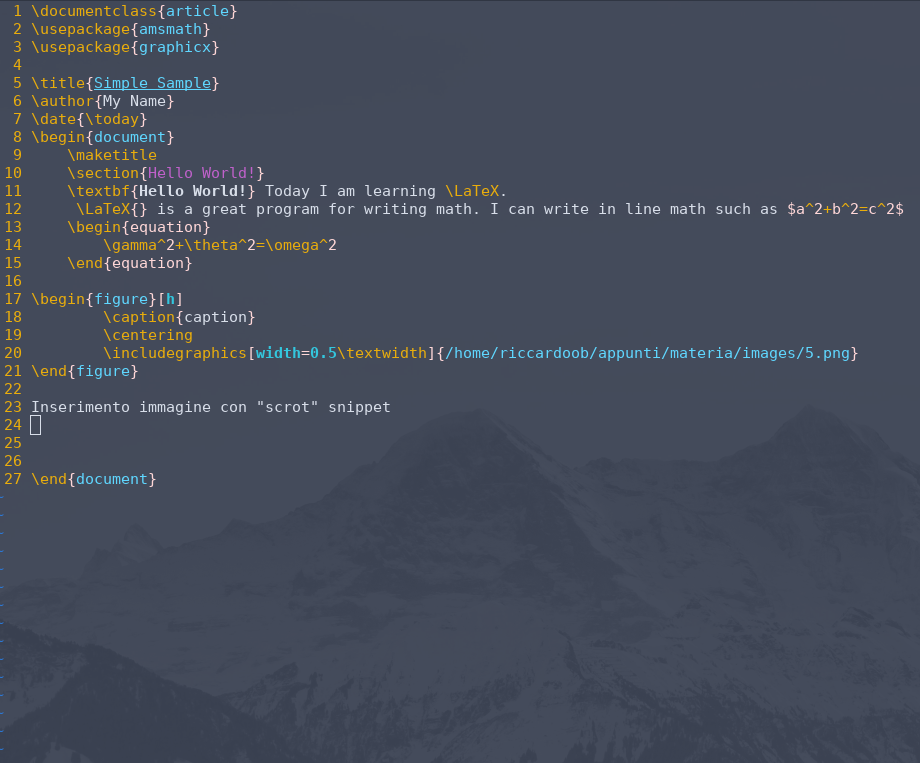
\includegraphics[width=0.7\linewidth]{/home/riccardoob/appunti/linguaggi/images/12.png}
    \end{subfigure}

\end{figure}

\subsubsection{Caso generale}
Nel caso bottom-up, in presenza di più stati finali:
\begin{itemize}
    \item si assume come (sotto)scopo $S_k$ uno stato finale per volta
    \item si scrivono le regole bottom-up corrispondenti
    \item si esprime il linguaggio complessivo come unione dei vari sotto-linguaggi, definendo lo \underline{scopo globale} come $S \rightarrow S_1\ |\ S_2\ |\ \cdots\ |\ S_n$
\end{itemize}



\chapter{Riconoscitori con PDA}

Un RSF \underline{non può riconoscere} un linguaggio di tipo 2, ha un limite intrinseco alla capacità di memorizzazione: non riesce a riconoscere frasi che richiedano di memorizzare una parte di lunghezza non nota a priori.

\textbf{Esempio}: bilanciamento delle parentesi $L = {(^n c )^n, n \ge 0}$, $G = {S \rightarrow (S)\ |\ c}$

In questo linguaggio il prefisso $(^n$ non ha lunghezza limitabile a priori.

\section{Push-Down Automaton (PDA)}
Un PDA è un RSF con aggiunto uno stack, con stack non ci si riferisce a una struttura dati fisica ma a un suo modello astratto, ovvero una sequenza di simboli, definito in modo tale che si possa operare soltanto su quello in "cima".

Il PDA legge un simbolo d'ingresso e transita in un nuovo stato, in più a ogni passo altera lo stack, producendo una nuova configurazione.

Un PDA può prevedere $\varepsilon$-mosse, ovvero transizioni spontanee che manipolano lo stack senza consumare simboli in ingresso.

Un PDA è una sestupla:

{\centering
$\langle A,\ S,\ S_0,\ sfn,\ Z,\ Z_0\rangle$\par}
dove:
\setlist{nosep}
\begin{itemize}
    \item $A$ = alfabeto
    \item $S$ = insieme degli stati
    \item $S_0$ = stato iniziale $\in S$
    \item $sfn: (A\cup \varepsilon) \times S \times Z \rightarrow W$
    \item $Z$ = alfabeto dei \underline{simboli interni} 
    \item $Z_0 \in Z$ = simbolo iniziale sullo stack
\end{itemize}
\setlist{}

\begin{figure}[H]
    \caption{Struttura PDA}
    \centering
    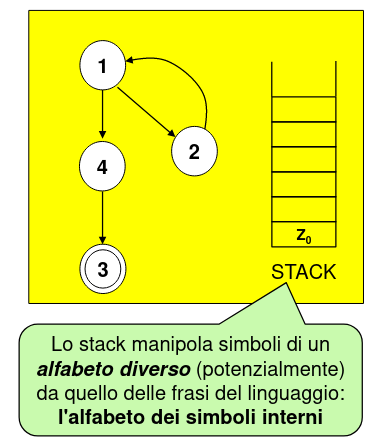
\includegraphics[width=0.4\textwidth]{/home/riccardoob/appunti/linguaggi/images/13.png}
\end{figure}

Il linguaggio \underline{accettatto} da un PDA è definibile in 2 modi equivalenti:
\begin{itemize}
    \item \textbf{Criterio dello stato finale}: il linguaggio accettato è l'insieme di tutte le stringhe di ingtesso che portano il PDA in uno degli stati finali.
    \item \textbf{Criterio dello stack vuoto}: il linguaggio accettato è definito come l'insieme di tutte le stringhe di ingresso che portano il PDA nella configurazione di \textit{stack vuoto}.
\end{itemize}

La funzione sfn, dati:
\begin{itemize}
    \item un \textit{simbolo in ingresso} $a\in A$
    \item lo \textit{stato attuale} $s\in S$
    \item il simbolo interno attualmente al \textit{top dello stack} $z\in Z$
\end{itemize}
opera come segue:
\begin{itemize}
    \item \textbf{consuma} il simbolo di ingresso $a$
    \item effettua il \textbf{POP} dello dallo stack, prelevando il simbolo $z$
    \item porta l'automa in stato futuro $s' = sfn(a, s, z)_{\prod S}$
    \item effettua una \textbf{PUSH} sullo stack di zero o più simboli interni $z'\in Z$\\ $z' = sfn(a, s, z)_{\prod S}$
\end{itemize}

Si consideri il linguaggio generato da:
\begin{itemize}
    \item $A = \{0, 1, c\}$
    \item $P = \{S \rightarrow 0\ S\ 0\ |\ 1\ S\ 1\ |\ c\}$
    \item $L = \{\texttt{word}\  c\ \texttt{word}^R\}$
\end{itemize}

Definiamo il PDA come segue:
\begin{itemize}
    \item $A = \{0, 1, c\}$
    \item $S = \{Q1=S_0, Q2\}$
    \item $Z = \{Zero, Uno, Centro\}$
\end{itemize}

\begin{figure}[H]
    \centering
    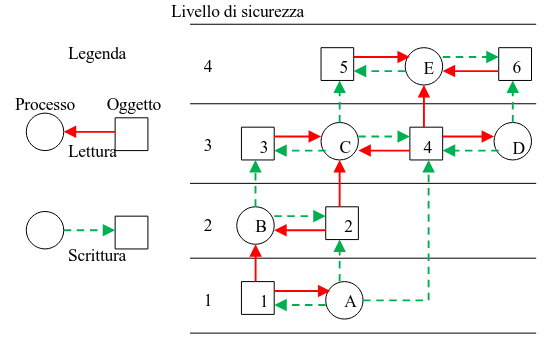
\includegraphics[width=0.5\textwidth]{/home/riccardoob/appunti/linguaggi/images/14.png}
\end{figure}

\subsection{PDA non deterministici}
Anche un PDA può essere non deterministico: in tal caso, la funzione $sfn$ produce insiemi di elementi $W$ ($W$ sottoinsieme finito di $S \times Z^*$).

Ad esempio, il PDA tale che $sfn(Q_0, a, Z) = \{(Q_1, Z_1)(\cdots)(Q_k, Z_k)\}$ è \textbf{non deterministico} in quanto l'automa, nello stato $Q_0$, con simbolo interno in cima allo stack $Z$ e ingresso $a$ ha \underline{più di uno stato futuro possibile} in base alla evoluzione cambia anche il se di simboli da porre nello stack.

\noindent
\textbf{TEOREMA}\\
La classe dei linguaggi riconosciuti da un PDA non-determistico coincide con la classe dei linguaggi context-free: perciò qualunque linguaggio context-free può sempre essere riconosciuto da un opportuno PDA.

É possibile rinunciare al determinismo?\\
In generale no:

\noindent
\textbf{TEOREMA}\\
Esistono linguaggi context-free riconoscibili soltanto da PDA non-deterministici.

ma in molti casi di interesse pratico esistono linguaggi context-free riconoscibili da PDA deterministici: \underline{linguaggi context-free deterministici}. 


\subsection{PDA deterministici}
Cosa serve per ottenerlo?

Viste le condizioni precedenti, non deve succedere che l'automa, in dato stato $Q_0$, con simbolo in cima allo stack $Z$ e ingresso $x$ possa:
\begin{itemize}
    \item portarsi in \underline{più stati futuri} 
        $sfn(Q_i, x, Z) = \{(Q_1, Z_1), (\cdots), (Q_k, Z_k)\}$
    \item optare se leggere o non leggere il simbolo di ingresso $x$ a causa della presenza di entrambe le mosse $sfn(Q_i, x, Z)$ e $sfn(Q_i, \varepsilon, Z)$
\end{itemize}

\underline{Unendo}, \underline{intersecando} o \underline{concatenando} linguaggi deterministici,  non necessariamente si ottiene un linguaggio deterministico.

I \underline{complemento} di un linguaggio è deterministico.

Con $L$ linguaggio deterministico e $R$ linguaggio regolare, il \underline{linguaggio quoziente}  $L/R$ (insieme di stringhe di $L$ private di suffisso regolare) è deterministico.

Con $L$ linguaggio deterministico e $R$ linguaggio regolare, il \underline{concatenamento} $L.R$ (insieme di stringhe di $L$ cun suffisso regolare) è deterministico.

\subsubsection{Sottoclassi particolari}
Per un PDS \textbf{deterministico}:
\begin{itemize}
    \item il criterio dello \underline{stack vuoto} risulta meno potente del criterio \underline{stati finali}
    \item una limitazione sul numero di stati intenro o sul numero di configurazioni finali riduce l'insieme dei linguaggi riconoscibili
    \item l'assenza di $\varepsilon$-mosse riduce l'insieme dei linguaggi riconoscibili
\end{itemize}


\subsection{Realizzazione di PDA deterministici}
Possibilità di seguire la definzione, ma non molto pratico.

Si adotta un approccio che manipoli uno stack con la stessa logica di un PDA, dove lo stack è la vera differenza, ad esempio una macchina virtuale che abbia uno stack può essere fatta funzionare come PDA, opportunamente pilotata.

Si potrebbe controllare "a mano" lo stack, oppure in modo automatico attraverso le \underline{chiamate ricorsive di funzioni}, dove sono già gestiti stack relativi alla ricorsione.

\subsubsection{Top-Down Recursive-Descent Parsing}

Con l'\textbf{analisi ricorsiva discendente} si introduce \underline{una funzione per ogni metasimbolo} della grammatica, e la si chiama ogni volta che si icontra quel metasimbolo.

Ogni funzione copre le regole di quel metasimbolo, ossia riconosce il sotto-linguaggio corrispondente:
\begin{itemize}
    \item termina normalmente (o segno di successo) se incontra simboli coerenti
    \item abortisce (o restituisce un segno di fallimento) se incontra simboli non coerenti
\end{itemize}

\subsubsection{Esempio}

Il solito linguaggio $L = \{\texttt{word}\ c\ \texttt{word}^n\}$, alfabeto $A = \{0,\ 1,\ c\}$ e regole $S \rightarrow 0\ S\ 0\ |\ 1\ S\ 1\ |\ c$. 

\begin{itemize}
    \item Introdurre tante funzioni quanti i metasimboli, qui una sola $S()$.
    \item Chiamare una funzione ogni volta che si incontra il suo metasimbolo
    \item Ogni funzione deve coprire le regole di quel metasimbolo
        \begin{itemize}
            \item se il simbolo d'ingresso è 0 $\rightarrow$ seguire la prima regola
            \item se il simbolo d'ingresso è 1 $\rightarrow$ seguire la seconda regola
            \item se il simbolo d'ingresso è c $\rightarrow$ seguire la terza regola
        \end{itemize}
\end{itemize}

Nel caso della prima regola, consumiamo il carattere di ingresso 0, invochiamo la funzione $S()$ e consumiamo un nuovo carattere d'ingresso e verifichiamo che sia 0.

Se la verifica ha esito positivo, significa che la funzone ha incontrato simboli coerenti con le proprie regole.

Se la verifica ha esito negativo, significa che la funzione ha incontrato simboli che non corrispondono alle sue regole.

\underline{\textbf{finisci slide esempio 24-28!!!!!!!!!!!!!!!!!!!!!!!!!!!!!!!!!!!!!!!!!!!!!!!!!!!!!!!!!!!!!!!!!!!!!!!!!!!!}}

\subsection{Separare motore e grammatica}
Applicare l'analisi ricorsiva discendente è un processo meccanico, che tuttavia introduce informazioni cablate nel codice, difficili da aggiornare.

É possibile separare il \textbf{motore}, invariante rispetto alle regole, dalle \underline{regole della grammatica}; si presta a questo scopo la \underline{tabella di parsing}, simile alla tabella delle transizioni di un RSF, indica però la prossima \textit{produzione} da applicare.

Il motore prenderà singole decisioni consultando questa tabella.

\subsubsection{Parsing tables - esempi deterministici}

\paragraph{Linguaggio} $L = \{\texttt{word}\ c\ \texttt{word}^n\}$

\begin{figure}[H]
    \centering
    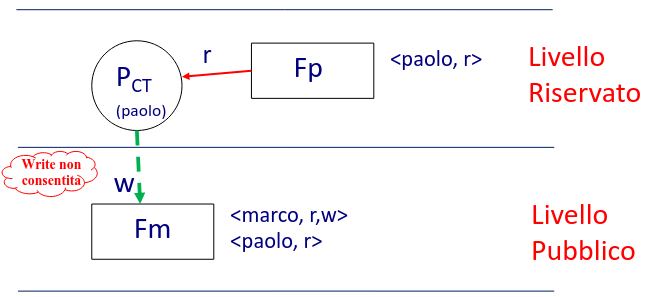
\includegraphics[width=0.8\textwidth]{/home/riccardoob/appunti/linguaggi/images/15.png}
\end{figure}

\paragraph{Linguaggio} $L = \{\texttt{if}\ \texttt{c}\ \texttt{then}\ \texttt{cmd}\ (\ \texttt{endif}\ |\ \texttt{else}\ \texttt{cmd}\ )\ \}$ 

\paragraph{Produzioni} $S \rightarrow \texttt{if}\ \texttt{c}\ \texttt{then} \ \texttt{cmd} \ \texttt{X} $, $\texttt{X}  \rightarrow \texttt{endif}\ |\ \texttt{else}\ \texttt{cmd} $ 

\begin{figure}[H]
    \centering
    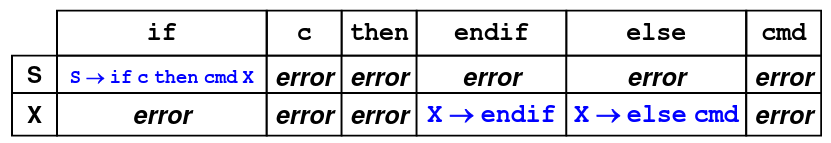
\includegraphics[width=0.8\textwidth]{/home/riccardoob/appunti/linguaggi/images/16.png}
\end{figure}

\subsection{Analisi ricorsiva discendente - vantaggi e limiti}
Vantaggi
\begin{itemize}
    \item immediata scrittura del riconoscitore
    \item migliore leggibilità a modificabilità del codice
    \item facilitata inserzione di azioni nella fase di analisi
\end{itemize}
Svantaggi
\begin{itemize}
    \item non sempre applicabile
    \item funzionale solo se non esistono ambiguità sulla regola da applicare
\end{itemize}

Si individua una sottoclasse di grammatiche context-free che garantisce il determinismo dell'analisi sintattica.

Per rendere deterministica l'analisi ricorsiva, si rende necessario avere una visione del \textit{passato} dell'analisi (simboli consumati fino a quel punto) e una del \textit{futuro}, generalmente un solo carattere in avanti.

\section{Grammatiche $LL(k)$}
Si definiscono \textit{grammatica $LL(k)$} quelle che sono analizzabili in modo deterministico:
\begin{itemize}
    \item procedendo \textit{left to right}
    \item applicando \textit{left-most derivation}
    \item guardando avanti al più \textit{k} simboli
\end{itemize}

Ricoprono un posto fondamentale le grammatiche LL(1), ovvero quelle in cui basta guardare un simbolo in avanti per operare in modo deterministico.

\subsubsection{Esempio}
Si consideri la grammatica
\begin{itemize}
    \item $\texttt{VT}\ =\ \{\texttt{p},\ \texttt{q},\ \texttt{a},\ \texttt{b},\ \texttt{d},\ \texttt{x},\ \texttt{y}\}$
    \item $\texttt{VN}\ =\ \{\texttt{S},\ \texttt{X},\ \texttt{Y}\}$
\end{itemize}

Produzioni
\begin{equation*}
    \begin{aligned}
        &\texttt{S} \rightarrow \texttt{p}\ \texttt{X}\ &&|\ \texttt{q}\ \texttt{Y}\\
        &\texttt{X} \rightarrow \texttt{a}\ \texttt{X}\ \texttt{b}\ &&|\ \texttt{x}\\
        &\texttt{Y} \rightarrow \texttt{a}\ \texttt{Y}\ \texttt{d}\ &&|\ \texttt{y}
    \end{aligned}
\end{equation*}

Le parti \textbf{destre} delle produzioni di uno stesso meta simbolo, iniziano tutte con un simbolo terminale diverso, è sufficiente guardare avanti di un carattere per scegliere con certezza la produzione per scegliere con certezza la produzione con cui proseguire l'analisi.

Creando la parsing table, si nota che ogni cella contiene una sola produzione, quindi non si hanno ambiguità sulle prossime mosse da fare, è facile vedere che il parser è deterinistico.

\begin{figure}[H]
    \centering
    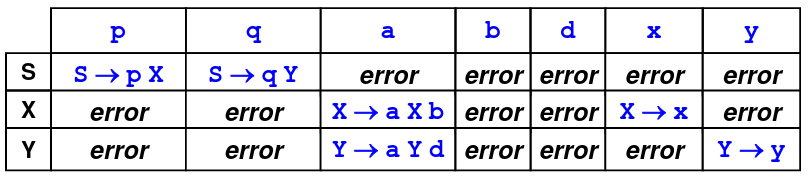
\includegraphics[width=0.8\textwidth]{/home/riccardoob/appunti/linguaggi/images/17.png}
\end{figure}

La frase di inzio deve essere completa oppure può essere parziale? Nel caso in cui si voglia imporre che la frase deve essere finale occorre imporre una regola \textit{top-level} che specifica che la frase deve terminare con \texttt{\$}, carattere che rappresenta il fine stringa/linea/file del tipo $\texttt{Z} \rightarrow \texttt{S}\ \$$ .

\subsection{Starter Symbol Set}
Spesso le parti destre delle produzioni di uno stesso metasimbolo non iniziano tutte con un simbolo terminale, non è chiaro quali siano gli input ammissibili.

Occorre ridefinire il concetto di simbolo iniziale $\rightarrow$ \underline{Starter Symbols Set}.

Lo starter symbols set della riscrittura $\alpha$ è l'insieme
\begin{equation*}
    SS(\alpha) = \{ a \in \texttt{VT}\ |\ \alpha \xrightarrow{}\mathrel{\vphantom{\to}^*} a\ \beta\}, \texttt{ con } \alpha \in V^+ \texttt{ e } \beta \in V^*
\end{equation*}

In sostanza gli starter symbols sono le iniziali di una forma di frase $\alpha$, ricavate applicando con più produzioni.
L'operatore $*$ cattura il caso limite in cui $\alpha \in VT$, ossia già terminale, e non richiede di applicare derivazioni.

Per includere anche il caso $\alpha \rightarrow \varepsilon$, si introduce l'insieme
\begin{equation*}
\texttt{FIRST}(\alpha ) = \texttt{trunc}_1(\{x \in VT^*\ |\ \xrightarrow{}\mathrel{\vphantom{\to}^*}\}), \texttt{ con } \alpha \in V^*
\end{equation*}

dove $\texttt{trunc}_1$ denota il troncamento della stringa al primo elemento.

Generalizzando la regola precendete, condizione necessaria perché una grammatica sia $LL(1)$ è che gli \textit{start symbols} relativi alle parti destre di uno stesso metasimbolo siano disgiunti.

\textbf{\underline{Esempi 44-52???????????????????????????????????????????????????????????????????????????????????????????}} 

É possibile capire in modo più rapido se una grammatica è $LL(1)$?

Due opzioni:
\begin{itemize}
    \item agire sulla parsing table, formalizzando il concetto di \textbf{blocco annullabile} e integrando nella tabella l'informazione sulle stringhe che possono scomparire.
    \item ampliare la nozione di starte symbols set con i \underline{Director Symbols} set (o \underline{Look-Ahed} set)
\end{itemize}

\underline{\textbf{inserisci slide 55-67!!!!!!!!!!!!!!!!!!!!!!!!!!!!!!!!!!!!!!!!!!!!!!!!!!!!!!!!!!!!!!!!!!!!!!!!!!!!!!!!!!!!!!!!!!!!!!!1}}  














\chapter{Dai riconoscitori agli interpreti}

\subsubsection{Dai puri riconoscitori...}
Finora si sono considerati soltanto \textit{puri riconoscitori}, che:
\begin{itemize}
    \item accettano in ingresso una stringa di caratteri
    \item riconoscono se essa appartiene a un linguaggio
\end{itemize}

\begin{figure}[H]
    \centering
    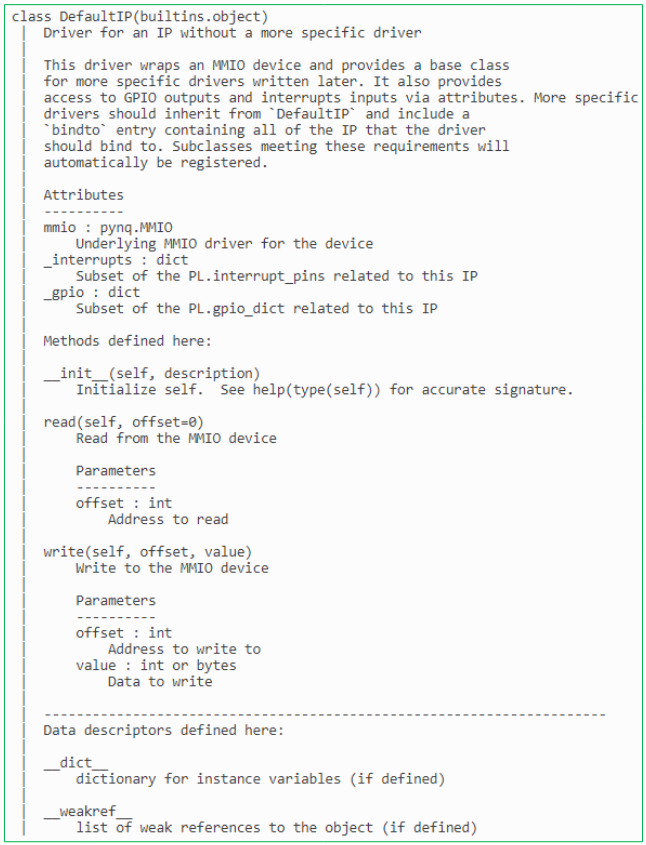
\includegraphics[width=0.8\textwidth]{/home/riccardoob/appunti/linguaggi/images/18.png}
\end{figure}

La risposta è sempre di tipo booleano, non ha importanza \textit{come} si arriva a stabilire la correttezza.

\subsubsection{...agli interpreti}
Un \textbf{interprete} è più di un puro riconoscitore, riconosce una stringa ma esegue anche azioni in base al significato (\textit{semantica}) della frase analizzata.

In questo caso diventa importante la \underline{sequenza di derivazione}.

\section{Interprete}

\subsection{Struttura}
Un interpreste è solitamente basasto su due componenti:
\begin{itemize}
    \item analizzatore lessicale, \textbf{scanner} o \textit{lexer}
    \item analizzatore sintattico-semantico, \textbf{parser}
\end{itemize}

\begin{figure}[H]
    \centering
    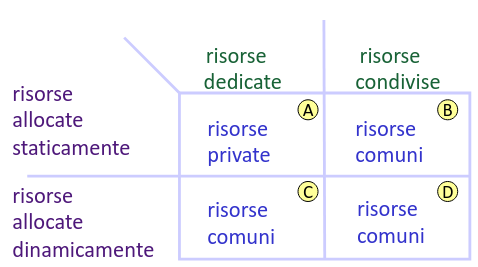
\includegraphics[width=0.8\textwidth]{/home/riccardoob/appunti/linguaggi/images/19.png}
\end{figure}

Lo scanner analizza le parti \textit{regolari} dei linguaggi, fornendo al parser singoli token già aggregati.

Il parser riceve dallo scanner i token, considerati come elementi terminali del suo linguaggio per valutare la correttezza della loro sequenza: opera sulle parti context free del linguaggio.

\subsection{Analisi lessicale}
L'analisi lessicale è la fase in cui si individuano le singole parole (token) che compongono la frase. Questa azione viene svolta raggruppando i singoli caratteri dell'input secondo \textbf{produzioni regolari} associate alle diverse possibili \textbf{categorie} lessicali.

L'analizzatore lessicale categorizza i token osservando in quale stato finale del RSF si ritrova.

\begin{figure}[H]
    \centering
    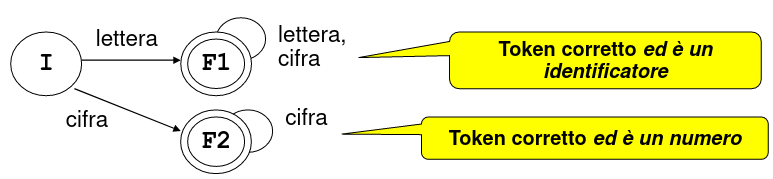
\includegraphics[width=0.8\textwidth]{/home/riccardoob/appunti/linguaggi/images/20.png}
\end{figure}

\subsection{Parole chiave}
Cablare ogni dettaglio nella struttura del RSF non è una buona strategia in quanto renderebbe estremamente complicato il riconoscitore.

\begin{figure}[H]
    \caption{Esempio riconoscimento identificatore if}
    \centering
    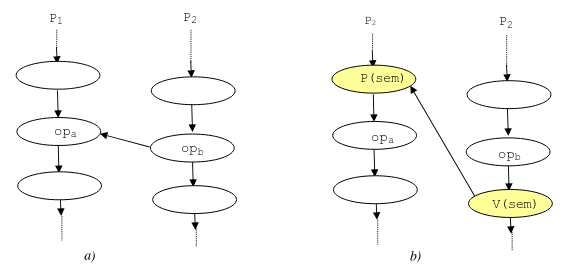
\includegraphics[width=0.7\textwidth]{/home/riccardoob/appunti/linguaggi/images/21.png}
\end{figure}

\subsection{Tabelle}
Per evitare di cablare le parole chiave, simboli etc. nella struttura del RSF, conviene agire diversamente:
\begin{itemize}
    \item categorizzare prima le parole chiave come identificatori
    \item ricategorizzare poi consultando opportune tabelle che incapsulano il dettaglio del linguaggio
    \begin{itemize}
        \item tabella \textit{parole chiave}
        \item tabella \textit{simboli}
    \end{itemize}
\end{itemize}

\subsection{Analisi sintattica top-down}
In caso di grammatiche $LL(1)$, una tecnica semplice per costruire il riconoscitore è l'analisi top-down ricorsiva discendente.

Per passare da un puro riconoscitore a un interprete occorre propagare qualcosa di più di un si o no, come ad esempio un \textbf{albero}, per una valutazione differita.

\section{Caso di studio - espressioni aritmetiche}
Si supponga di voler riconoscere espressioni aritmetiche con le quattro operazioni \textbf{+ * - /}.

\begin{figure}[H]
    \centering
    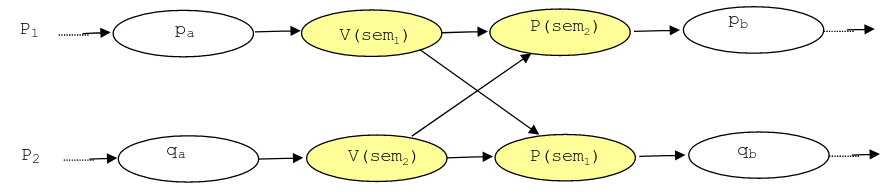
\includegraphics[width=0.8\textwidth]{/home/riccardoob/appunti/linguaggi/images/22.png}
\end{figure}

Un puro riconoscitore deve solo dire se sono corrette, ma un interprete deve anche dire:
\begin{itemize}
    \item se il dominio sono gli \textit{interi} il risultato può essere un valore int
    \item se il dominio sono i \textit{reali} il risultato può essere un valora double
    \item se l'obiettivo è la \textit{valutazione differita}, il risultato può essere un opportuno oggetto (albero)
\end{itemize}

\subsection{Analisi del dominio}

\subsubsection{Sintassi}
La notazione classica insegnata identifica i quattro operatori con i seguenti simboli: $+$, $-$, $\times$, $:$.

Sono stati sostituiti dagli informatici con $+$, $-$, $*$, $/$, spesso vengono anche usate le parentesi per esprimere una priorità associativa.

\subsubsection{Semantica}
Nel dominio aritmetico usuale:
\begin{itemize}
    \item i \textit{valori numerici} si assumono espressi in notazione \textbf{posizionale} su base dieci
    \item il significato inteso dei quattro \textit{operatori} è quello di somma, sottrazione, moltiplicazione, divisione
    \item si denotano le nozioni di priorità e associatività
    \begin{itemize}
        \item \textbf{priorità} fra operatori diversi, moltiplicativi prioritari su quelli additivi
        \item \textbf{associatività} tra operatori equiprioritari, solitamente si associa a sinistra
    \end{itemize}
\end{itemize}

\subsection{Grammatica per le espressioni}
Consideriamo il linguaggio $E(G)$ relativo alla seguente grammatica per espressioni aritmetiche;
\setlist{nosep}
\begin{itemize}[label={}]
    \item $\texttt{VN} = \{ \texttt{EXP}\}$
    \item $\texttt{VT} = \{+, *, -, :, \texttt{num}\}$
    \item $S = \texttt{EXP}$
    \item $P = \{$
    \begin{itemize}[label={}]
        \item $\texttt{EXP} := \texttt{EXP} + \texttt{EXP}$
        \item $\texttt{EXP} := \texttt{EXP} - \texttt{EXP}$
        \item $\texttt{EXP} := \texttt{EXP} * \texttt{EXP}$
        \item $\texttt{EXP} := \texttt{EXP} : \texttt{EXP}$
        \item $\texttt{EXP} := \texttt{num}$ 
    \end{itemize}
    \item $\}$
\end{itemize}
\setlist{}
É una grammatica ambigua, la semantica è informale: se \texttt{EXP} è un numero, l'espressione denota un intero e il valore dell'espression coincide con quello del numero.

\subsection{Una grammatica a "strati"}
É possibile dare una struttura \textit{gerarchica} alle espressioni, esprimendo così intrinsicamente priorità e associatività degli operatori.
\setlist{nosep}
\begin{itemize}[label={}]
    \item $\texttt{VN} = \{ \texttt{EXP}, \texttt{TERM}, \texttt{FACTOR}\}$
    \item $\texttt{VT} = \{+, *, -, :, (, ), \texttt{num}\}$
    \item $S = \texttt{EXP}$
    \item $P = \{$
    \begin{itemize}[label={}]
        \item $\texttt{EXP} := \texttt{TERM}$
        \item $\texttt{EXP} := \texttt{EXP} + \texttt{TERM}$
        \item $\texttt{EXP} := \texttt{EXP} - \texttt{TERM}$
        \item $\texttt{TERM} := \texttt{FACTOR}$
        \item $\texttt{TERM} := \texttt{TERM} * \texttt{FACTOR}$
        \item $\texttt{TERM} := \texttt{TERM} : \texttt{FACTOR}$
        \item $\texttt{FACTOR} := \texttt{num}$
        \item $\texttt{FACTOR} := ( \texttt{EXP})$
    \end{itemize}
    \item $\}$
\end{itemize}
\setlist{}
Ogni strato considera \textit{terminali} gli elementi linguistici definiti in altri strati:
\begin{itemize}
    \item \texttt{EXP} considera terminali $+$, $-$ e \texttt{TERM}
    \item \texttt{TERM} considera terminali $*$, $:$ e \texttt{FACTOR}
    \item \texttt{FACTOR} considera terminali \texttt{num}, $($, $)$, e \texttt{EXP}
\end{itemize}

Le \textit{somme} e \textit{sottrazioni} aggregano i \underline{termini}, le \textit{moltiplicazioni} e \textit{divisioni} aggregano i \underline{fattori} e i \textit{fattori} sono entità \underline{atomiche}.

\begin{figure}[H]
    \caption{Priorità operatori}
    \centering
    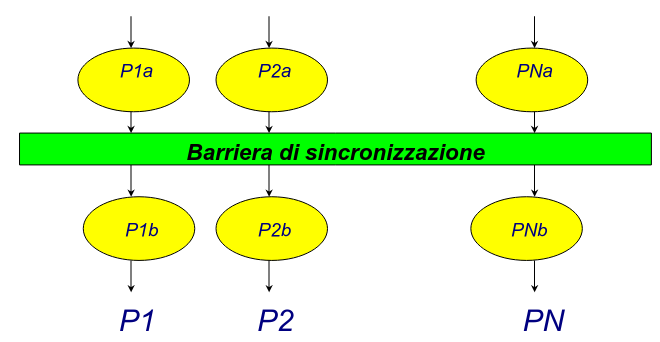
\includegraphics[width=0.8\textwidth]{/home/riccardoob/appunti/linguaggi/images/23.png}
\end{figure}

\subsubsection{Esempi}

\begin{multicols}{2}
    Frase:\\
    \noindent
    $(0111 + 0011) * 0010$\\
    Albero di derivazione
    \begin{multicolfigure}
        \centering
        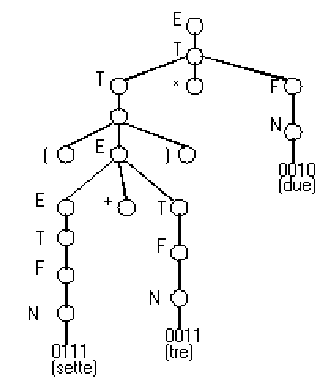
\includegraphics[width=0.7\textwidth]{/home/riccardoob/appunti/linguaggi/images/24.png}
    \end{multicolfigure}
    \columnbreak
    Frase:\\
    \noindent
    $0111 + 0011 + 0010$\\
    Albero di derivazione
    \begin{multicolfigure}
        \centering
        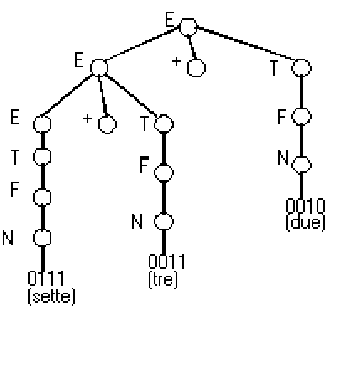
\includegraphics[width=0.7\textwidth]{/home/riccardoob/appunti/linguaggi/images/25.png}
    \end{multicolfigure}
\end{multicols}

La grammatica individuata è \textit{ricorsiva a sinistra} per esprimere la corretta associatività, tuttavia è incompatibile con l'analisi ricorsiva discendente, utile per la costruzione del parser.

\subsection{Variante 1 - Associativa a destra}
Se si riscrivono le regole in forma ricorsiva a destra, ovvero invertendo \texttt{TERM} e \texttt{EXP} e \texttt{FACTOR} e \texttt{TERM}, si otterrebbe una associatività inversa rispetto a quella usuale.

Ad esempio l'espressione $7 - 3 - 2$ verrebbe derivata come $7 - ( 3 - 2 )$ anziché come $( 7 - 3 ) - 2$.

\setlist{nosep}
\begin{itemize}[label={}]
    \item $\texttt{VN} = \{ \texttt{EXP}, \texttt{TERM}, \texttt{FACTOR}\}$
    \item $\texttt{VT} = \{+, *, -, :, (, ), \texttt{num}\}$
    \item $P = \{$
    \begin{itemize}[label={}]
        \item $\texttt{EXP} := \texttt{TERM}$
        \item $\texttt{EXP} := \texttt{TERM} + \texttt{EXP}$
        \item $\texttt{EXP} := \texttt{TERM} - \texttt{EXP}$
        \item $\texttt{TERM} := \texttt{FACTOR}$
        \item $\texttt{TERM} := \texttt{FACTOR} * \texttt{TERM}$
        \item $\texttt{TERM} := \texttt{FACTOR} : \texttt{TERM}$
        \item $\texttt{FACTOR} := \texttt{num}$
        \item $\texttt{FACTOR} := ( \texttt{EXP})$
    \end{itemize}
    \item $\}$
\end{itemize}
\setlist{}


\subsection{Variante 2 - Non associativa}
Si potrebbe anche fare a meno dell'associatività, mantenendo però lo stesso ordine di priorità. Queste regole non usano ricorsione, ne destra ne sinistra, risolvendo il problema \textit{obbligando a usare le parentesi}.

\setlist{nosep}
\begin{itemize}[label={}]
    \item $\texttt{VN} = \{ \texttt{EXP}, \texttt{TERM}, \texttt{FACTOR}\}$
    \item $\texttt{VT} = \{+, *, -, :, (, ), \texttt{num}\}$
    \item $P = \{$
    \begin{itemize}[label={}]
        \item $\texttt{EXP} := \texttt{TERM}$
        \item $\texttt{EXP} := \texttt{TERM} + \texttt{TERM}$
        \item $\texttt{EXP} := \texttt{TERM} - \texttt{TERM}$
        \item $\texttt{TERM} := \texttt{FACTOR}$
        \item $\texttt{TERM} := \texttt{FACTOR} * \texttt{FACTOR}$
        \item $\texttt{TERM} := \texttt{FACTOR} : \texttt{FACTOR}$
        \item $\texttt{FACTOR} := \texttt{num}$
        \item $\texttt{FACTOR} := ( \texttt{EXP})$
    \end{itemize}
    \item $\}$
\end{itemize}
\setlist{}

\section{Dalla grammtica al parser}
\subsection{Ricorsione sinista e analisi top-down}
Il riconoscitore è un PDA, perché la grammatica ha self-embedding, il problema è che la sintassi delle espressioni include produzioni \textit{ricorsive sinistra}, quindi questa non è una grammatica $LL(1)$.

\subsubsection{Trasformazione della grammatica}
Si procede riconsiderando i sotto-linguaggi generati dai diversi strati:
\setlist{nosep}
\begin{itemize}[label={}]
    \item $\texttt{L(EXP)} = \texttt{TERM} \pm \texttt{TERM} \pm \texttt{TERM} \dots$
    \item $\texttt{L(TERM)} = $*/:$ \texttt{FACTOR} $*/:$ \texttt{FACTOR} \dots$
    \item $\texttt{L(FACTOR)} = \texttt{num}\ |\ \texttt{(EXP)}$
\end{itemize}
\setlist{}

Continuiamo mappando le espressioni individuate seconda la notazione EBNF:
\setlist{nosep}
\begin{itemize}[label={}]
    \item \texttt{EXP} = \texttt{TERM} $\{(+ | -) \texttt{TERM}\}$
    \item \texttt{TERM} = \texttt{FACTOR} $\{(* | :) \texttt{FACTOR}\}$
\end{itemize}
\setlist{}
Queste regole non presentano più ricorsione esplicita, descrivono un processo computazionale iterativo.

Questa è una grammatica $LL(1)$, in quanto è analizzabile con una tecnica ricorsiva discendente e hanno start symbols set distinti.

Si può esplicitare inserendo un termine:
\setlist{nosep}
\begin{itemize}[label={}]
    \item \texttt{EXP} = \texttt{TERM} \texttt{AFTERTERM}
    \item \texttt{AFTERTERM} = $\varepsilon\ |\ +$\texttt{EXP}$\ |\ -$\texttt{EXP} 
    \item \texttt{TERM} = \texttt{FACTOR} \texttt{AFTERFACTOR}
    \item \texttt{AFTERFACTOR} = $\varepsilon\ |\ *$\texttt{TERM}$|\ :$\texttt{TERM}
\end{itemize}
\setlist{}
Questa è una grammatica $LL(1)$ ma è anche ricorsiva a destra, non verrà quindi utilizzata operativamente ma solo per la verifica $LL(1)$

\subsubsection{Schema parser}
Si effettua una analisi ricorsiva discendente:
\begin{itemize}
    \item procedura o funzione per ogni simbolo non terminale
    \item invocazione ricorsiva solo per il caso con self-embedding
\end{itemize}

Tutte le funzioni restituiscono un \textit{boolean}, nel caso di puro riconoscitore, oppure un valore o oggetto nel caso di parser completi con valutazione.

Ogni funzione dovrebbe terminare quando incontra un simbolo che non appartiene al sotto-linguaggio di sua pertinenza.

\begin{lstlisting}[language=java]
    public boolean parseExp() {
        boolean t1 = parseTerm();
        while (currentToken != null) {
            if (currentToken.equals("+"))
\end{lstlisting}

\textbf{\_\_\_\_\_\_\_\_\_\_\_\_\_\_\_\_\_\_\_\_\_\_\_\_\_\_\_\_\_\_\_\_\_\_\_\_\_\_\_\_\_\_\_\_\_\_\_\_\_\_\_inserisci codice slide 37-39\_\_\_\_\_\_\_\_\_\_\_\_\_\_\_\_\_\_\_\_\_\_\_\_\_\_\_\_\_\_\_\_\_\_\_\_\_\_\_\_\_\_\_\_\_\_\_\_\_\_\_}

\subsubsection{Una architettura di sistema}
Si passa ora a definira una architettura di supporto per il parser, come ad esempio concretizzare il concetto di \textbf{token} e astrarre lo scanner per leggere la stringa e definire il modello di interazione tra parser e scanner.

Si potrebbe, ad esempio, utilizzare una variabile privata \texttt{currentToken}, una classe \texttt{MyScanner} per tokenizzare la stringa e una classe \texttt{Token} che incapsula una stringa.

\textbf{\_\_\_\_\_\_\_\_\_\_\_\_\_\_\_\_\_\_\_\_\_\_\_\_\_\_\_\_\_\_\_\_\_\_\_\_\_\_\_\_\_\_\_\_\_\_\_\_\_\_\_inserire codice 42-46\_\_\_\_\_\_\_\_\_\_\_\_\_\_\_\_\_\_\_\_\_\_\_\_\_\_\_\_\_\_\_\_\_\_\_\_\_\_\_\_\_\_\_\_\_\_\_\_\_\_\_}

\section{Dal parser al valutatore}
Finora abbiamo definito come:
\begin{itemize}
    \item dato il \textit{linguaggio} desiderato, trovare una \textit{grammatica} adatta a descriverlo
    \item data la grammatica, scrivere un puro \textit{riconoscitore} per tale linguaggio
\end{itemize}
manca:
\begin{itemize}
    \item data la grammatica, scrivere un \textbf{parser} completo che effettui una \textbf{valutazione}
\end{itemize}
serve:
\begin{itemize}
    \item la specifica della semantica che il parser dovrà applicare
\end{itemize}

\subsection{Specificare la semantica}
É necessario un modo sistematico e formale stabilire con precisione il \textbf{significato} di ogni possibile frase di un linguaggio: se il linguaggio è \textit{infinito} serve una notazione finita applicabile a infinite frasi.

Un metodo può essere qello di definire una \textit{funzione di interpretazione}:
\begin{itemize}
    \item \underline{dominio}, ovvero il linguaggio
    \item \underline{codominio}, ovvero l'insieme dei possibili significati
\end{itemize}

\subsection{Semantica denatoziale}
Quando la semantica di un lingauggio è espressa in questo modo si parla di \textbf{semantica denotazionale}.

L'idea principale è quella di associare a ogni \textit{regola sintattica} una \textbf{regola semantica}.

Nel caso delle espressioni aritmetiche la sintassi prevede \texttt{Exp}, \texttt{Term} e \texttt{Factor}, quindi la semantica prevederà le funzioni \texttt{fExp}, \texttt{fTerm} e \texttt{fFactor}.

\begin{itemize}
    \item \texttt{fExpr(s)}
    \begin{itemize}
        \item \texttt{fTerm(s)} se \texttt{s} non contiene ne $+$ ne $-$
        \item \texttt{fExpr(s1)}$+$\texttt{fTerm(s2)}, se \texttt{s} ha la forma \texttt{s1}$+$\texttt{s2}
        \item \texttt{fExpr(s1)}$-$\texttt{fTerm(s2)}, se \texttt{s} ha la forma \texttt{s1}$-$\texttt{s2}
    \end{itemize}
    \item \texttt{fTerm(s)}
    \begin{itemize}
        \item \texttt{fFactor(s)} se \texttt{s} non contiene ne $*$ ne $:$
        \item \texttt{fTerm(s1)}$\times$\texttt{fFactor(s2)} se \texttt{s} ha la forma \texttt{s1}$*$\texttt{s2}
        \item \texttt{fTerm(s1)}$/$\texttt{fFactor(s2)} se \texttt{s} ha la forma \texttt{s1}$:$\texttt{s2}
    \end{itemize}
    \item \texttt{fFactor(s)}
    \begin{itemize}
        \item \texttt{fFactor(innerExp)} se \texttt{s} ha la forma \texttt{(innerExp)}
        \item \texttt{valueof(num)}, se \texttt{s} ha la forma \texttt{num}
    \end{itemize}
\end{itemize}

\begin{figure}[H]
    \centering
    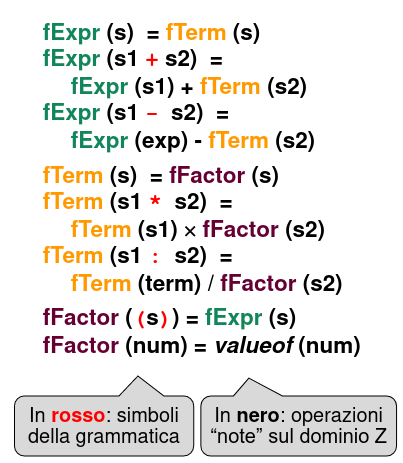
\includegraphics[width=0.4\textwidth]{/home/riccardoob/appunti/linguaggi/images/32.png}
\end{figure}
\subsubsection{Esempio}
\begin{figure}[H]
    \centering
    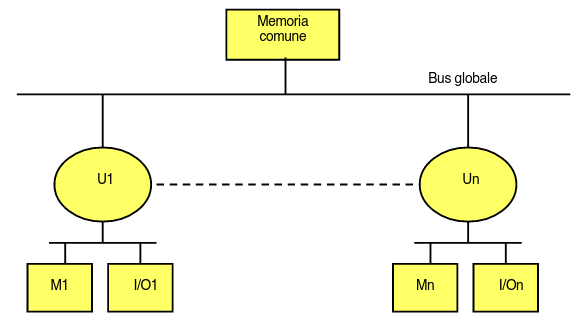
\includegraphics[width=0.7\textwidth]{/home/riccardoob/appunti/linguaggi/images/33.png}
\end{figure}

\subsubsection{Schema interprete}
Ogni funzione analizza il sotto-linguaggio di pertinenza:
\begin{itemize}
    \item \texttt{parseExp} analizza \texttt{L(EXP)}, per il quale $+$, $-$ e \texttt{TERM} sono l'alfabeto terminale
    \item \texttt{parseTerm} analizza \texttt{L(TERM)}, per il quale $*$, $:$ e \texttt{FACTOR} sono l'alfabeto terminale
    \item \texttt{parseFactor} analizza \texttt{L(FACTOR)}, il cui alfabeto terminale è costituito da $($, $)$ e \texttt{EXP}
\end{itemize}

\textbf{\_\_\_\_\_\_\_\_\_\_\_\_\_\_\_\_\_\_\_\_\_\_\_\_\_\_\_\_\_\_\_\_\_\_\_\_\_\_\_\_\_\_\_\_\_\_\_\_\_\_\_inserisci codice slide 64-67\_\_\_\_\_\_\_\_\_\_\_\_\_\_\_\_\_\_\_\_\_\_\_\_\_\_\_\_\_\_\_\_\_\_\_\_\_\_\_\_\_\_\_\_\_\_\_\_\_\_\_}
\subsection{Elevamento a potenza}
Se si volesse aggiungere l'elevamento a potenza?

Si introduce l'operatore \texttt{\^}, che denota un elevamento a potenza: $3*4^2$ si scrive \texttt{3*4\^{}2} 

Questo operatore ha priorità maggiore di tutti gli altri e si considera la sua associatività è a destra, ovvero si interpreta $4^{2^3}$ o \texttt{4\^{}2\^{}3} come $4^8$.

Si aggiunge un nuovo "strato" alla grammatica a strati definita in precedenza:
\begin{figure}[H]
    \centering
    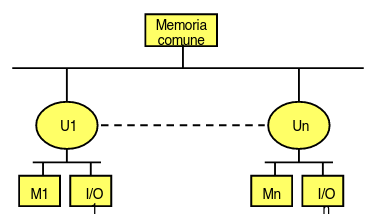
\includegraphics[width=0.4\textwidth]{/home/riccardoob/appunti/linguaggi/images/34.png}
\end{figure}

\textbf{\_\_\_\_\_\_\_\_\_\_\_\_\_\_\_\_\_\_\_\_\_\_\_\_\_\_\_\_\_\_\_\_\_\_\_\_\_\_\_\_\_\_\_\_\_\_\_\_\_\_\_inserisci codice slide 70-72\_\_\_\_\_\_\_\_\_\_\_\_\_\_\_\_\_\_\_\_\_\_\_\_\_\_\_\_\_\_\_\_\_\_\_\_\_\_\_\_\_\_\_\_\_\_\_\_\_\_\_}

\section{Rappresentare le frasi}
Manca soltanto una rappresentazione intermedia della frase interpretata per poter "risolverla" successivamente, qui entrano in gioco gi \textbf{alberi sintattici}.

\subsection{Alberi sintattici astratti}
Si potrebbe usare dirattamente l'\textit{albero di derivazione}, ma darebbe luogo a una rappresentazione ridondante.

Conviene adottare un albero più \textit{compatto}, che contenga solo i nodi indispensabili, la soluzione è il \textbf{Abstract Syntax Tree} (AST).

Tipologie di nodi non indispensabili:
\begin{itemize}
    \item i nodi terminali (foglie) non legati a niente di significativo sono ridondanti e possono essere ignorati, le foglie 
    \item le foglie che esauriscono la loro funzione dopo il parser, nelle espressioni le parentesi
    \item le foglie che hanno un unico nodo figlio
\end{itemize}

\begin{multicols}{2}    
    \begin{multicolfigure}
        \centering
        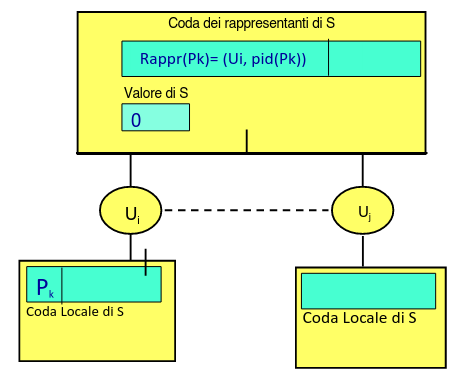
\includegraphics[width=0.5\textwidth]{/home/riccardoob/appunti/linguaggi/images/35.png}
    \end{multicolfigure}
    \columnbreak
    \begin{multicolfigure}
        \centering
        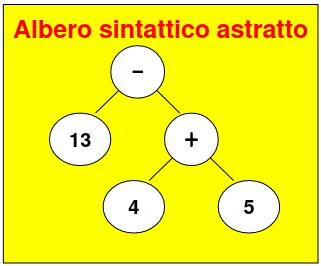
\includegraphics[width=0.5\textwidth]{/home/riccardoob/appunti/linguaggi/images/36.png}
    \end{multicolfigure}
\end{multicols}

\subsubsection{Esempio espressioni}

Nel caso delle espressioni, l'AST è così definito
\begin{itemize}
    \item ogni \textbf{operatore} è un nodo con due figli
    \begin{itemize}
        \item figlio sinistro è il primo operando
        \item figlio destro è il secondo operando
    \end{itemize}
    \item i valori numerici sono le foglie
\end{itemize}

La rappresentazione è sempre univoca, quindi la struttura dell'albero fornisce intrinsicamente l'ordine corretto di valutazione.

Si tenta ora di estendere il parser per generare l'opportuno AST, per farlo è necessario stabilire quali e quanti tipi di nodo diversi si hanno.

\begin{figure}[H]
    \centering
    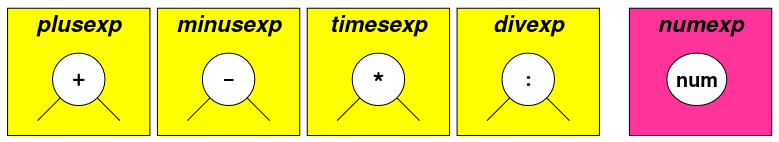
\includegraphics[width=0.6\textwidth]{/home/riccardoob/appunti/linguaggi/images/37.png}
\end{figure}

\subsection{Sintassi astratta}
Per descrivere formalmente questi nodi si utilizza una \textbf{sintassi astratta}, ad esempio i nodi in considerazione possono essere rappresentanti con la seguente sintassi astratta

\setlist{nosep}
\begin{itemize}[label={}]
    \item \texttt{EXP} = \texttt{EXP} $+$ \texttt{EXP}
    \item \texttt{EXP} = \texttt{EXP} $-$ \texttt{EXP}
    \item \texttt{EXP} = \texttt{EXP} $*$ \texttt{EXP}
    \item \texttt{EXP} = \texttt{EXP} $:$ \texttt{EXP}
    \item \texttt{EXP} = \texttt{num}
\end{itemize}
\setlist{}

\subsubsection{Una possibile implementazione dell'AST}
\textbf{\_\_\_\_\_\_\_\_\_\_\_\_\_\_\_\_\_\_\_\_\_\_\_\_\_\_\_\_\_\_\_\_\_\_\_\_\_\_\_\_\_\_\_\_\_\_\_\_\_\_\_inserisci codice slide 86-89\_\_\_\_\_\_\_\_\_\_\_\_\_\_\_\_\_\_\_\_\_\_\_\_\_\_\_\_\_\_\_\_\_\_\_\_\_\_\_\_\_\_\_\_\_\_\_\_\_\_\_}

Si passa ora alla nuova implementazione del parser che include la nuova architettura ad AST.

\textbf{\_\_\_\_\_\_\_\_\_\_\_\_\_\_\_\_\_\_\_\_\_\_\_\_\_\_\_\_\_\_\_\_\_\_\_\_\_\_\_\_\_\_\_\_\_\_\_\_\_\_\_inserisci codice slide 91-93\_\_\_\_\_\_\_\_\_\_\_\_\_\_\_\_\_\_\_\_\_\_\_\_\_\_\_\_\_\_\_\_\_\_\_\_\_\_\_\_\_\_\_\_\_\_\_\_\_\_\_}

\section{Architettura interprete}
\begin{figure}[H]
    \centering
    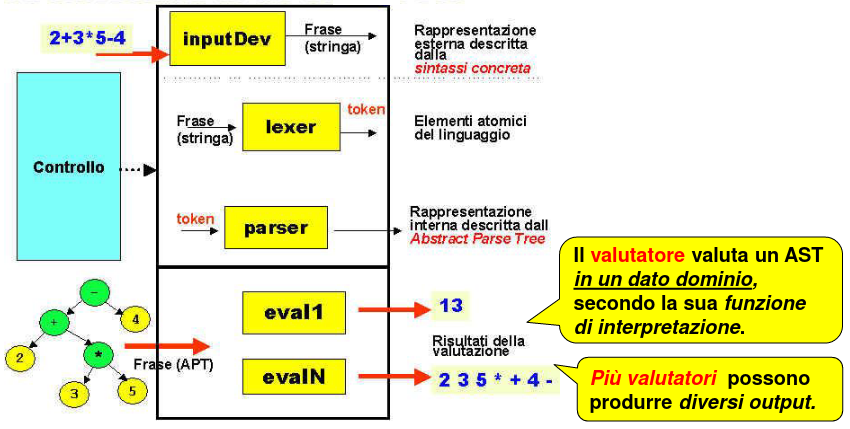
\includegraphics[width=0.8\textwidth]{/home/riccardoob/appunti/linguaggi/images/40.png}
\end{figure}
Si è arrivati al punto nel quale sono state definite strategie per:
\begin{itemize}
    \item dato il linguaggio desiderato, trovare una \textit{grammatica} adatta
    \item data la grammatica, scrivere il \textit{puro riconoscitore} per il linguaggio
    \item data la grammatica, scrivere un \textit{parser} completo che valuti e generi l'albero
\end{itemize}

manca da \textbf{valutare l'albero sintattico} dopo la sua generazione.

\section{Valutazione di alberi}
Esistono diverse modalità per analizzare una albero, la teoria degli alberi introduce il concetto di \underline{visita}:
\begin{itemize}
    \item \textit{pre-order}, radice $\rightarrow$ figli (da sx a dx)
    \item \textit{post-order}, figli (da sx a dx) $\rightarrow$, radice
    \item \textit{in-order}, figlio sx $\rightarrow$ radice $\rightarrow$ figlio dx
\end{itemize}

Nel nostro dominio delle espressioni aritmetiche, queste metodologie si traducono in:
\begin{itemize}
    \item notazione \textbf{prefissa}
    \item notazione \textbf{postfissa}
    \item notazione \textbf{infissa} classica
\end{itemize}

Con la notazione postfissa si presta perfettamente alla traduzione in codice per un elaboratore, in quanto fornisce prima gli operandi e successivamente cosa farne.

Idealmente si caricherebbero gli operandi su un registro, ma essendo questi limitati si utilizza lo \textbf{stack}.

Evoluzione dello stack:
\begin{multicols}{2}
    \begin{multicolfigure}
        \centering
        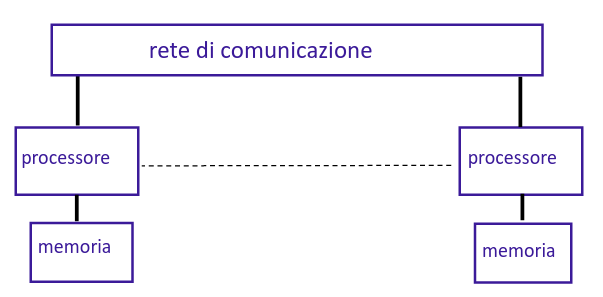
\includegraphics[width=0.45\textwidth]{/home/riccardoob/appunti/linguaggi/images/38.png}
    \end{multicolfigure}
    
    \begin{multicolfigure}
        \centering
        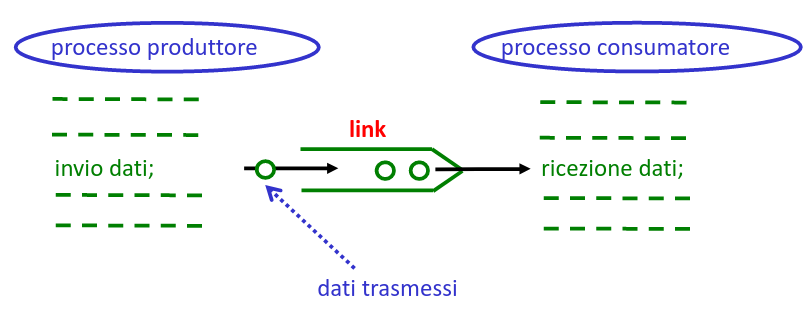
\includegraphics[width=1\textwidth]{/home/riccardoob/appunti/linguaggi/images/39.png}
    \end{multicolfigure}
\end{multicols}

\section{Valutatore}
Il valutatore incorpora la funziona di valutazione, che deve \textbf{visitare} l'albero applicando la corretta \textit{semantica} a seconda del nodo visitato.

\subsection{Implementazione}
É necessario implementare un metodo \texttt{eval()} che calcola il valore di una espressione, conviene introdurre questo metodo nella classe astratta dell'AST, per poi specializzare la sua implementazione per ogni tipo di nodo.

\begin{lstlisting}[language=java]
    public abstract class Exp {
       public abstract int eval();
    }
\end{lstlisting}

Si utilizza quindi una metodologia completamente object oriented, senza creare una funzione piena di if..else per scegliere l'azione da eseguire, questo approccio comporta tuttavia la decentralizzazione della valutazione, con conseguente impatto in caso di necessità di modifiche.

\subsubsection{Stile a oggetti}
\begin{lstlisting}[language=java]
    abstract class Exp {
        abstract public int eval();
    }
    ...
    class PlusExp extends OpExp {
        public PlusExp(Exp l, Exp r) {
            super(l,r);
        }
        public String myOp() {
            return "+";
        }
        public int eval() {
            return left.eval() + right.eval();
        }
    }
    ...
    class NumExp extends Exp {
        int val;
        public NumExp(int v) {
            val = v;
        }
        public int eval() {
            return val;
        }
    }
\end{lstlisting}

\subsubsection{Confronto}
\begin{itemize}
    \item Metodologia \textbf{funzionale}
    \begin{itemize}
        \item \textit{PRO}: facilitata l'introduzione di \textbf{nuove interpretazioni}, basta scrivere una nuova \texttt{eval2()}
        \item \textit{CONTRO}: rende più oneroso introdurre una \textbf{nuova produzione}, impatta tutte le funzioni di interpretazione
    \end{itemize}
    \item Metodologia \textbf{object oriented}
    \begin{itemize}
        \item \textit{PRO}: facilita l'aggiunta di \textbf{nuove produzioni}, basta aggiungere nuova classe, con relative eval
        \item \textit{CONTRO}: rende oneroso introdurre \textbf{nuove intepretazioni}, impatta tutte le classi della tassonomia nell'introduzione del relativo metodo
    \end{itemize}
\end{itemize}

\subsubsection{Cosa scegliere}
Solitamente un linguaggio di programmazione ha una \textit{grammatica fissa} ma richiede \textit{molteplici interpretazioni} delle frasi (per analisi della semantica, type checking, code generation etc.); per questo l'approccio funzionale sembrerebbe il più adatto.

É necessario unire i pro delle due metodologie, a questo compito si presta perfettamente il \textbf{pattern Visitor}, che ci permette di incapsulare la \textit{logica d'interpretazione} in una entità di livello più alto.

\subsection{Visitor come interprete}
Questo pattern realizza la logica di interpretazione in modo coerente all'approccio a oggetti: cattura \textbf{una} logica di interpretazione, centralizzandola in un unico posto.

Nel caso delle espressioni si possono realizzare
\begin{itemize}
    \item una classe base astratta (o interfaccia) \texttt{Visitor}
    \item visitor per \textit{stampare} le espressioni $\rightarrow$ \texttt{ParExpVisitor}
    \item visitor per \textit{calcolare} le espressioni $\rightarrow$ \texttt{EvalVisitor}
    \item visitor per tradurre le espressioni sotto forma di \textit{codice}
    \item ...
\end{itemize}

\begin{multicols}{2}
    \begin{multicolfigure}
        \centering
        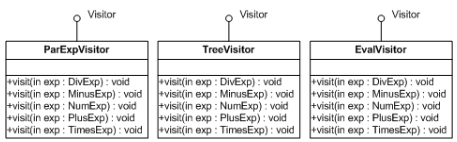
\includegraphics[width=1\textwidth]{/home/riccardoob/appunti/linguaggi/images/41.png}
    \end{multicolfigure}
    \begin{multicolfigure}
        \centering
        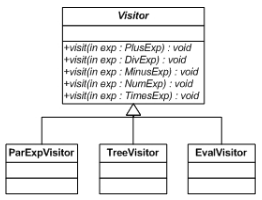
\includegraphics[width=0.7\textwidth]{/home/riccardoob/appunti/linguaggi/images/42.png}
    \end{multicolfigure}
    
\end{multicols}

\textbf{\_\_\_\_\_\_\_\_\_\_\_\_\_\_\_\_\_\_\_\_\_\_\_\_\_\_\_\_\_\_\_\_\_\_\_\_\_\_\_\_\_\_\_\_\_\_\_\_\_\_\_inserisci codice slide 162-173\_\_\_\_\_\_\_\_\_\_\_\_\_\_\_\_\_\_\_\_\_\_\_\_\_\_\_\_\_\_\_\_\_\_\_\_\_\_\_\_\_\_\_\_\_\_\_\_\_\_\_}

























\chapter{Estensione: assegnamenti, ambienti, sequenze}

\section{Assegnamento}
Ogni linguaggio di programmazione introduce le nozioni di \textbf{variabili} e \textbf{assegnamento}.

L'assegnamento non è una uguaglianza o equazione, ma denota l'azione di prendere la destra dell'uguale e metterla all'interno della sinistra dell'uguale, considerando come valori le variabili sulla destra e contenitori le variabili sulla sinistra.

Si deduce che il simbolo di variabile ha significato diverso tra la destra e la sinistra dell'operatore.

\subsection{L-Value vs R-Value}
Si definisce quindi la distinzione tra l-value e r-value:
\begin{itemize}
    \item \textbf{l-value}: il significato della variabile a sinistra è la variabile \textit{in quanto tale}
    \item \textbf{r-value}: il significato della variabile a destra è il \textit{contenuto} della variabile
\end{itemize}

Sorge inoltre la questione dell'\textit{assegnamento distruttivo/non distruttivo}, è possibile cambiare il valore associato in precedenza a un simbolo di variabile?

Nei linguaggi \textit{imperativi} l'assegnameto è distruttivo, nei linguaggi \textit{logici} si ha una trasparenza referenziale dove un simbolo ha sempre lo stesso valore.

\section{Environment}
Per esprimere al meglio la semantica dell'assegnamento, occorre introdurre il concetto di \textbf{environment}, inteso come \textit{insieme di coppie} \texttt{(simbolo, valore)}


































\chapter{Multi-Paradigm Programming: parser espressioni in Prolog}

Il motore Prolog contiene un suo scanner e un suo parser usato per interpretare la sua sintassi di regole.

L'obiettivo è quello di mappare la nostra sintassi "sopra" alla sua per riutilizzare le strutture già definite.

Cosa abbiamo già:
\begin{itemize}
    \item tre dei quattro operatori sono già \textit{operatori infissi} leciti in Prolog
\end{itemize}

Cosa manca:
\begin{itemize}
    \item l'operatore \texttt{:} è diverso in quanto Prolog usa la barra \texttt{/}
    \item le parentesi tonde sono già intercettate dal parser di Prolog
\end{itemize}

\subsection{Definizione nuovi operatori}
Per definire un nuovo operatore infisso in Prolog basta porre all'inizio della teoria logica la dichiarazione
\begin{minted}[bgcolor=lightgray,framesep=2mm,baselinestretch=1.2,fontsize=\footnotesize]{Prolog}
:- op(livellopriorità, associatività, operatore)
\end{minted}

\begin{itemize}
    \item livellopriorità: numero che esprime la priorità dell'operatore
    \item associatività: atomo che esprime se l'operatore è infisso o pre/postfisso e la sua associatività
    \item operatore: è il nuovo operatore da dichiarare
\end{itemize}
\begin{minted}[bgcolor=lightgray,framesep=2mm,baselinestretch=1.2,fontsize=\footnotesize]{Prolog}
:- op(400, yfx, ':')
\end{minted}

\subsection{Problema delle parentesi tonde}
Non si possono utilizzare parentesi tonde dato che sono utilizzate da Prolog, sostituiamo quindi le tonde con le parentesi quadre, anch'esse già utilizzate da prolog per le liste (già riconosciute e bilanciate).

Il prezzo sarà minimo, in quanto consiste solo nella differenza della forma delle parentesi, esistono inoltre tecniche per mascherarle.

\subsection{Espressioni in Prolog}
La semantica denotazionale definita esprime già tutte le regole "pattern oriented", sono direttamente trasferirle in Prolog.


\begin{minted}[bgcolor=lightgray,framesep=2mm,baselinestretch=1.2,fontsize=\footnotesize]{Prolog}
fExpr(Term) :- fTerm(Term).
fExpr(Exp+Term) :- fExpr(Exp), fTerm(Term).
fExpr(Exp-Term) :- fExpr(Exp), fTerm(Term).
fTerm(Factor) :- fFactor(Factor).
fTerm(Term*Factor) :- fTerm(Term), fFactor(Factor).
fTerm(Term:Factor) :- fTerm(Term), fFactor(Factor).
fFactor([Exp]) :- fExpr(Exp).
fFactor(num) :- number(Num).
\end{minted}

Le funzioni sono solo sintassi, per ora non hanno nessun significato.

\subsection{Dal riconoscitore al valutatore}
Per sintetizzare il valutatore è necessario:
\begin{itemize}
    \item estendere la testa delle regole aggiungendo un \textit{argomento per restituire il risultato}
    \item estendere il corpo delle regole, ricavando i \textit{valori} e \textit{combinandoli} in modo appropriato alla semantica
\end{itemize}

Per il trattamento dei numeri, Prolog utilizza soltanto il concetto di numeri reali, e attraverso il predicato \texttt{is} si può applicare la semantica dei numeri naturali.

\begin{minted}[bgcolor=lightgray,framesep=2mm,baselinestretch=1.2,fontsize=\footnotesize]{prolog}
evalExpr(Term, Value) :- evalTerm(Term, Value).
evalExpr(Exp+Term, Value) :- evalExpr(Exp, Value1),
                             evalTerm(Term, Value2),
                             Value is Value1 + Value2.
evalExpr(Exp-Term, Value) :- evalExpr(Exp, Value1),
                             evalTerm(Term, Value2),
                             Value is Value1 - Value2.
evalTerm(Factor, Value) :- evalFactor(Factor, Value).
evalTerm(Term*Factor, Value) :- evalTerm(Term, Value1),
                                evalFactor(Factor, Value2),
                                Value is Value1 * Value2.
evalTerm(Term:Factor, Value) :- evalTerm(Term, Value1),
                                evalFactor(Factor, Value2),
                                Value is Value1 / Value2.
evalFactor([Exp], Value) :- evalExpr(Exp, Value).
evalFactor(Num, Num) :- number(Num).
\end{minted}

\section{Parser ibrido con 2p-kt}
Java si occupa di:
\begin{itemize}
    \item visualizzare finestre di dialogo per richiedere stringa di input
    \item sostituire parentesi tonde con quadre
    \item \textit{creare} un \textbf{motore Prolog}, configurandolo con l'opportuna \textbf{teoria} e \textbf{interrogarlo} con l'espressione
    \item recuperare e visualizzare il risultato della valutazione
\end{itemize}
tuProlog si occupa di
\begin{itemize}
    \item interpretare e valutare l'espressione data
\end{itemize}

\subsection{Primi passi per utilizzare il Prolog engine}

Leggere la teoria logica (input o file)
\begin{minted}[bgcolor=lightgray,framesep=2mm,baselinestretch=1.2,fontsize=\footnotesize]{java}
ClausesReader theoryReader = ClausesReader.getWithDefaultOperators();
Theory theory = theoryReader.readTheory(input);
\end{minted}

Ottenere una istanza di \texttt{SolverFactory}, per ottenere il un solver adeguato
\begin{minted}[bgcolor=lightgray,framesep=2mm,baselinestretch=1.2,fontsize=\footnotesize]{java}
SolverFactory solverFactory = ClassicSolverFactory.INSTANCE;
\end{minted}

Costruire tramite la factory il solver, passando la teoria
\begin{minted}[bgcolor=lightgray,framesep=2mm,baselinestretch=1.2,fontsize=\footnotesize]{java}
Solver solver = solverFactory.solverWithDefaultBuiltins(theory);
\end{minted}

\subsection{TermParser}
Il \texttt{TermParser} è il componente che effettua il parsing dei termini, deve quindi riconoscere tutti gli operatori, anche quelli definiti custom.

É possibile costruire un \texttt{TermParser} con i giusti operatori "a mano" oppure è possibile ottenere dal solver le definizioni trovate.

\subsubsection{Metodo 1}
\begin{minted}[bgcolor=lightgray,framesep=2mm,baselinestretch=1.2,fontsize=\footnotesize]{java}
OperatorSet myOpSet = OperatorSet.STANDARD.plus(new Operator(":", Specifier.YFX, 400));
TermParser termParser = TermParser.withOperators(myOpSet);
\end{minted}

\subsubsection{Metodo 2}

\begin{minted}[bgcolor=lightgray,framesep=2mm,baselinestretch=1.2,fontsize=\footnotesize]{java}
TermParer termParser = TermParser.withOperators(solver.getOperators())
\end{minted}

Per creare la query a partire dalla rappresentazione testuale
\begin{minted}[bgcolor=lightgray,framesep=2mm,baselinestretch=1.2,fontsize=\footnotesize]{java}
Struct query = termParser.parseStruct("evalExpr(" + queryText + ", Result)");
\end{minted}

















































\chapter{Strumenti per la generazione automatica di riconoscitori LL}

Esistono moltissimi strumenti chiamati \textit{parser generator}, o compiler compiler, questi, data una grammatica (annotata), producono automaticamente il riconsocitore in un linguaggi prescelto.

Alcuni seguono l'approccio LL, altri quello LR:
\begin{itemize}
    \item LL è efficiente e facilita l'aggiunta di azioni semantiche
    \item LR è più potente (vedi ricorsione sinistra) ma più complesso
\end{itemize}

Oltre alla generazione del perser tuttavia, è necessario integrarsi con strumenti di sviluppo, come impostare validazione, segnalazioni di errori, content assists, quick fix e altro.

\section{Domain-Specific Languages}
Al contrario dei GPL, General Purpose Languages, i \textbf{DSL} sono realizzati per essere utilizzati in \textbf{specifici domini applicativi}, non mirano a \textit{risolvere ogni problema} ma a offrire soluzioni efficaci per uno specifico ambito.

Esistono strumenti a supporto dei DSL, utili per la \textit{generazione automatica} dei DSL e del supporto, il più diffuso è \texttt{Xtext}.
























\end{document}
